% ==========================================
% ============= Dokumentklasse/Präaambel =============
% ==========================================
\documentclass[a4paper,12pt,twoside]{scrreprt}
\usepackage[left=2cm, right=2cm, top=2.5cm, bottom=2.5cm]{geometry}
\usepackage{float}
\usepackage{tikz}


%\usepackage[onehalfspacing]{setspace}\onehalfspacing 


%nicht einrücken nach jedem Absatz
%\setlength{\parindent}{0pt}


% ============= Packages =============
%PDF-Dokumentinformationen
\usepackage[
	pdftitle={Analyse der Lawinengefahr in Südtirol: Eine Bewertung des bestehenden Lawinenkatasters durch Gefahrenkartierung und Simulationen},
	pdfsubject={},
	pdfauthor={Jean Patrick Franzelin},
	pdfkeywords={},	
	%Links nicht einrahmen
	hidelinks
]{hyperref}


% ============= Standard Packages =============
\usepackage{wrapfig}
\usepackage[utf8]{inputenc}		%Paket um Sonderzeichen zu erhalten
\usepackage[ngerman]{babel}		%Paket um deutsche Gramatik zu erkennen
\usepackage[T1]{fontenc}		%Ausgabefonts	
\usepackage{subcaption} % Paket für subfigure-Umgebung%Paket um Bilder einbinden zu können
\graphicspath{{img/}}
\usepackage{fancyhdr}			%Paket für erweiterte Kopf- und Fußzeilen
\usepackage{lmodern}
\usepackage{color}
\usepackage{listings}   	%Paket für Code Listings
\usepackage{multirow}		%Paket um Zellen/Spalten in Tabellen zu verbinden
\usepackage{booktabs}		%Paket um verkitale und horizontale Linien in Tabellen einfacher zu erstellen
\usepackage{titletoc}		%Paket zur Manipulation des Inhaltsverzeichnis
\usepackage{tocbasic}		%Paket zur Manipulation des Inhaltsverzeichnis

%zusätzliche Schriftzeichen der American Mathematical Society
\usepackage{amsfonts}
\usepackage{amsmath}
\usepackage{amssymb}

\usepackage[printonlyused]{acronym}		%Paket für Abkürzungsverzeichnise
\usepackage{siunitx}					%Paket um mathematische Einheiten zu verwenden
\usepackage{hyperref}					%Paket für Links und Verweise im PDF-Dukument
\usepackage[toc,page]{appendix}			%Paket um Anhänge zu erstellen
\usepackage[utf8]{inputenc}
\usepackage[ngerman]{babel}
\usepackage{titletoc} % Paket für Inhaltsverzeichnisanpassungen
\usepackage{hyperref}
\usepackage[utf8]{inputenc}
\usepackage{booktabs} % Für schönere Tabellen
\usepackage{longtable} % Für Tabellen, die eine Seite überschreiten können
% Custom commands
\usepackage{float}
\newcommand{\supervisor}[1]{\def\thesupervisor{#1}}
\newcommand{\uselogo}[2]{\def\theuselogo{\includegraphics[#2]{#1}}}
\usepackage{amsmath}
\usepackage{booktabs} % Für bessere Linien in Tabellen
\usepackage[labelfont=bf]{caption} % Für fetten Tabellenbeschriftungsstil
\usepackage{tabularx} % Ermöglicht Tabellen mit automatischer Breitenanpassung
\usepackage{caption}  % Verbesserte Beschriftungsfunktionen
\usepackage[utf8]{inputenc}
\usepackage{enumitem}
\setlist[itemize]{itemsep=4pt, topsep=4pt, parsep=0pt}
\usepackage[ngerman]{babel}
\usepackage{booktabs}
\usepackage[round]{natbib} % Runde Klammern um das Jahr
\bibliographystyle{apalike} % oder ein anderer Stil, der Autor-Jahr-Zitate unterstützt
\usepackage{subcaption}
% ============= Inhaltsverzeichnis anpassen =============
%\usetocstyle{allwithdot}			%Style für das Inhaltsverzeichnis


% ============= Kopf- und Fußzeile =============
%Befehl um Authoren, einzelnen Seiten/Kapitel zuzuweisen
\renewcommand{\chaptermark}[1]{%
\markboth{\thechapter.\ #1}{}}
\newcommand{\TheAuthor}{}
\newcommand{\Author}[1]{\renewcommand{\TheAuthor}{#1}}

%Standartpagestyle
\pagestyle{fancy}
%L->left, C->center, R->right

%Pagestyle "fancy" (Alle Seiten außer Titelseite und Chaper-Seiten)
\fancyhf{}
\fancyhead[LE,RO]{}
\fancyhead[RE,LO]{Collaborative
Building Footprint Quality Assessment}
\fancyfoot[RE,LO]{\thepage}
\fancyfoot[CE,CO]{\slshape \TheAuthor}
\fancyfoot[LE,RO]{Universität Zürich}
\renewcommand{\headrulewidth}{0.4pt}
\renewcommand{\footrulewidth}{0.4pt}

%Pagestyle "rmplain" (Alle Seiten mit römischer Nummerierung)
\fancypagestyle{rmplain}
{
	\fancyhf{}
	\fancyfoot[RE,LO]{\thepage}
	\renewcommand\headrulewidth{0pt}
	\renewcommand\footrulewidth{0pt}
}

%Pagestyle "plain" (Alle Chapter-Seiten)
\fancypagestyle{plain}{
	\fancyhf{}
	\fancyhead[LE,RO]{}
	\fancyhead[RE,LO]{Collaborative
Building Footprint Quality Assessment}
	\fancyfoot[RE,LO]{\thepage}
	\fancyfoot[CE,CO]{\slshape \TheAuthor}
	\fancyfoot[LE,RO]{Universität Zürich}
	\renewcommand{\headrulewidth}{0.4pt}
	\renewcommand{\footrulewidth}{0.4pt}
}


% ============= Package Einstellungen & Sonstiges ============= 
%Besondere Trennungen
\hyphenation{De-zi-mal-tren-nung}


%Gliederungstiefen einstellen (Subsubsection freischalten wenn in {} 5 steht)
\setcounter{secnumdepth}{5}
\setcounter{tocdepth}{5}


% ==========================================
% ============= Dokumentbeginn =============
% ==========================================
\begin{document}
%Erste Seite ohne Kopf- und Fußzeile sowie Seitenzahl
\pagestyle{empty}
\begin{titlepage}
    \begin{flushright}
        \vspace*{0.1cm}
        
\includegraphics[width=0.25\textwidth]{img/logo_uzh} % top-right logo
    \end{flushright}
    
    \centering
    \vspace*{0.1cm}
    
    \textbf{Author:} \\
    Jean Patrick Franzelin \\
    
    \vspace{2cm}
    
    \textbf{\huge Towards AI-Assisted Building Footprint Quality Assessment in the Global South Using Vision and Multimodal Foundation Models} \\[1cm]
    
    \textbf{\LARGE Master's Thesis} \\
    
    \vspace{1cm}
    
    submitted in partial fulfillment of the requirements for the degree of \\
    \textit{Master of Science (MSc)} \\
    in \textit{Geography with specialization in Geoinformatics and GIScience} \\
    
    \vspace{1.2cm}
    
    submitted to the \\
    
    \vspace{1cm}
    
    \textbf{\Large University of Zurich (UZH)} \\
    \textbf{\large Department of Geography (GIUZ)} \\
    \textbf{\large Geographic Information Visualization and Analysis (GIVA) Group} \\
    
    \vspace{1cm}
    
    \textbf{Supervisors:} \\
    Dr. Tumasch Reichenbacher \\
    Dr. Yuchang Jiang \\

    \textbf{Faculty representative:} \\
    Prof. Dr. Sara Irina Fabrikant
    
    \vfill
    
    \textbf{Zurich, 2026} \\
    
\end{titlepage}
		%include{...} einbinden der einzelnen Kapitel ein


%Alle folgenden Seiten bis zu dem Befehl \pagenumbering{arabic} werden mit römischen Ziffern nummeriert
\pagenumbering{roman}


% \chapter*{...} creates a heading without a chapter number
\chapter*{Personal Declaration}\thispagestyle{rmplain}
\label{02_declaration_of_authorship}

 I hereby declare that the submitted thesis is the result of my own, independent work. All external sources are explicitly acknowledged in the thesis\\[1.5cm]

Date: \hrulefill\enspace Signature: \hrulefill

\newpage




%\include{03_vorwort}


\chapter*{Abstract}\thispagestyle{rmplain}
\addcontentsline{toc}{chapter}{Abstract}
\label{05_abstract}



\newpage





% ==========================================
% Inhaltsverzeichnis einfügen
% ==========================================
\tableofcontents\thispagestyle{rmplain}


% ==========================================
% Abbildungsverzeichnis einfügen
% ==========================================
\listoffigures\thispagestyle{rmplain}	
\addcontentsline{toc}{chapter}{Abbildungsverzeichnis}	%Verzeichnis im Inhaltsverzeichnis hinzufügen (erzwingen)	


% ==========================================
% Tabellenverzeichnis einfügen
% ==========================================
\listoftables\thispagestyle{rmplain}
\addcontentsline{toc}{chapter}{Tabellenverzeichnis}


% ============= Glossary einbinden ============= 
%%Befehl um Einheiten im Acronym ausgeben zu können
\newcommand{\acrosecondcolumn}[1]{\acroextra{\makebox[21mm][l]{#1}}}

% ============= Eingabe der Symbole und Abkürzungen ============= 
\chapter*{Abkürzungsverzeichnis}\thispagestyle{rmplain}
\addcontentsline{toc}{chapter}{Abkürzungsverzeichnis}
\label{sec:abkuerzungsverzeichnis}
\begin{acronym}[LONGEST]
	\acro{KDE}{K Desktop Environment}
	\acro{SQL}{Structured Query Language}
	\acro{Bash}{Bourne-again shell}
	\acro{JDK}{Java Development Kit}
	\acro{VM}{Virtuelle Maschine}
	%Falls eine Abkürzung in der Mehrzahl nicht einfach auf "s" endet muss das speziell eingestellt werden. 
	\acro{slmtA}{super lange mega tolle Abkürzung} %Einzahl
	\acroplural{slmtA}[slmtAs]{super lange mega tolle Abkürzungen} %Mehrzahl
\end{acronym}


\chapter*{Symbolverzeichnis}\thispagestyle{rmplain}
\addcontentsline{toc}{chapter}{Symbolverzeichnis}
\label{sec:symbolverzeichnis}
\begin{acronym}[LONGEST]
	\acro{temp}[$^\circ\text{C}$]{Europäische Einheit der Temperatur}
	\acro{mu}[$\mu$]{Reibungskoeffizient}
	\acro{pi}[$\pi$]{Kreiszahl}
	\acro{alpha}[$\alpha$]{Winkel zwischen $0^\circ\text{C}$ und $360^\circ\text{C}$}
	\acro{n}[$\mathbb{N}$]{Menge der natürlichen ganzen Zahlen}
	\acro{A}[\ensuremath{A}]{Oberfläche}
	%\acro{A}[\ensuremath{A}]{\acrosecondcolumn{$m^2$}Oberfläche}	%Darstellung mit Einheit
\end{acronym}		%Wenn man ein auf Acronymen basierendes Verzeichniss haben möchte


%Beendet eine Seite und erzwingt auf den nachfolgenden Seiten die Ausgabe aller Gleitobjekte (z.B. Abbildungen), die bislang definiert, aber noch nicht ausgegeben wurden. Dieser Befehl fügt, falls nötig, eine leere Seite ein, sodass die nächste Seite nach den Gleitobjekten eine ungerade Seitennummer hat. 
\cleardoubleoddpage
%\pagestyle{otherpagesthenplain}
%\pagestyle{fancy}


%Ab hier wird im Inhaltsverzeichnis wie gewohnt mit arabischen Zahlen nummeriert
\pagenumbering{arabic}
\pagestyle{fancy}

\section{Introduction}
\label{Introduction}


Extracting building footprints has long been an essential task in aerial imagery interpretation and GIScience, supporting applications such as disaster management, urban planning, and infrastructure monitoring \citep{Awrangjeb_AutomaticExtraction}. Accurate and up-to-date building footprints are not only required by national mapping agencies for maintaining topographic databases, but also play a critical role in crisis situations \citep{ZHENG_Buildingdamage}. However, vectorizing building footprints over large areas requires substantial manual effort. Mapping agencies must invest significant man-hours into digitizing and validating footprints, which naturally motivates the development of automated or semi-automated approaches \citep{rastogi2022automatic}.

Over the past decades, many different methods have been proposed \citep{ZHENG_Buildingdamage}, yet no approach has achieved 100 percent accuracy \citep{rastogi2022automatic}, largely due to the vast diversity of building shapes, materials, and architectural concepts.

These challenges have increasingly motivated the use of artificial intelligence and deep learning methods for automated building-footprint extraction. The topics of Artificial Intelligence, Machine Learning, Deep Learning, and Neural Networks are closely related and build on one another \citep{shiri2023comprehensive}. They can be understood as a nested hierarchy: neural networks form the foundation; machine learning builds upon them; deep learning represents a layered subset of machine learning; and artificial intelligence encompasses all of these concepts. In this work, the focus lies specifically on deep learning using pretrained transformer-based
foundation models.

With the recent development of artificial intelligence, researchers have increasingly explored foundation models instead of purely task-specific deep-learning architectures. The Vision Transformer (ViT) \citep{DosovitskiyTransformer} was among the first transformer-based models for vision tasks, demonstrating that attention mechanisms can effectively be applied to image recognition. Building on this idea, the Dense Prediction Transformer (DPT) \citep{ranftl2021visiontransformersdenseprediction} showed that transformers can also produce coherent global predictions for dense visual tasks.

More recently, research has moved toward integrating visual foundation models with multimodal large language models (MLLMs) \citep{wu2023multimodallargelanguagemodels}. These models combine visual and textual reasoning, offering new possibilities for interpreting spatial data. In GIScience, such approaches could enhance spatial reasoning and enable automated analysis of geospatial features beyond pixel-level classification \citep{Ji_2025_foundationGeospatiolreasoning}. Early studies have begun to explore such combinations, typically allowing the language model to guide, describe, or evaluate the visual model's segmentation process. This development is directly relevant for this thesis, where MLLM-based visual assessment is combined with SAM-based segmentation for selective building-footprint refinement.

This thesis takes a different approach. Instead of using a language model to directly control segmentation, a two-step framework is proposed in which the MLLM evaluates existing building polygons and supports selective refinement, thereby clearly separating assessment and correction. This follows an update-oriented geospatial workflow, where the aim is not to reconstruct an entire building dataset from scratch, but to identify and improve features that require correction \citep{Qin_changedetection}.

In the first stage, imperfect building polygons from Google Open Buildings serve as the starting point. These polygons are evaluated by a multimodal large language model, which identifies whether a building is visible, directs the case into the appropriate refinement path, and generates spatial prompts where required. In the second stage, a visual foundation model generates refined geometry candidates, which are subsequently converted and regularized into GIS-ready building polygons.

This design addresses key limitations of current end-to-end approaches, which typically require large labeled datasets and are difficult to adapt across regions or data domains. By decoupling assessment, segmentation, and correction, the proposed workflow enables clearer feedback loops and greater flexibility in integrating automated quality assurance into geospatial production processes.

The research gap addressed in this thesis lies in the limited transfer of such multimodal, feedback-driven AI approaches to GIScience, particularly for the automated quality assessment of vector-based building footprints.


\textbf{RQ1:} To what extent can a multimodal large language model support the visual quality assessment of existing vector-based building footprints?

\textbf{RQ2:} How effectively can MLLM-generated spatial prompts, combined with SAM-based segmentation and geometric post-processing, improve selected building-footprint geometries?

\textbf{RQ3:} How transferable is the proposed workflow across different geographic regions, building morphologies, and imagery conditions?


\Author{Jean Patrick Franzelin}
\chapter{Theoretical Background}

This chapter introduces the core concepts underlying this thesis, including building footprint extraction, deep learning architectures, multimodal large language models, and current approaches to quality assessment in GIScience.


\section{Geospatial Data Quality}
\label{sec:geospatial_data_quality}

Geospatial data quality describes the degree to which spatial data are suitable for a given purpose.
\cite{veregin1999data} states that quality usually refers to a high degree of craftsmanship; however, this concept becomes more difficult to apply to data, which lack physical characteristics. Instead, geospatial data quality is commonly described through abstract properties such as accuracy, completeness, consistency, and resolution \citep{veregin1999data}.
These concepts are formalized in the international standard \textit{Geographic information — Data quality} (ISO~19157-1:2023), which defines a structured framework for describing and documenting geospatial data quality \citep{ISO19157-1:2023}. The standard specifies five core quality elements: completeness, logical consistency, positional accuracy, temporal quality, and thematic quality. Related work often uses slightly different terminology. For example, \citep{Vieira_dataqualityindicators} and \cite{dataqualityinEarthobservation} refer to completeness, logical consistency, positional accuracy, temporal accuracy, and attribute accuracy, while also emphasizing the importance of lineage or provenance as an additional quality indicator.

Across several studies on geospatial data quality, the concept of \emph{fitness-for-use} is introduced \citep{dataqualityinEarthobservation, veregin1999data, Chrisman_Theerrorcomponenst, Vieira_dataqualityindicators}. Originating from quality engineering, this concept was later adopted in GIScience and describes a shift in responsibility from data producers to data consumers. Rather than assuming the existence of universally “high-quality” datasets, geospatial data are evaluated relative to their intended application. In this view, errors are considered inevitable, and data quality is understood as a multidimensional and task-dependent property. Consequently, transparent documentation of limitations, uncertainty, and provenance becomes essential. \cite{caprioli2003rules} further emphasize that GIS environments typically integrate spatial datasets of different origins and quality levels, often leaving the overall system accuracy undefined. They argue that while standards support interoperability and documentation, compliance alone does not guarantee quality, since standards cannot account for all application contexts. Instead, spatial data quality must ultimately be evaluated in terms of fitness-for-use, requiring both producer metadata and user-driven assessment. The authors also highlight practical challenges in GIS workflows, including quality loss during data conversion, scalability issues, and the difficulty of maintaining consistent accuracy across heterogeneous datasets.


High geospatial data quality is crucial because geospatial information is directly used to address real-world problems and to support decision-making processes \citep{GeospatialData_Selmy}. Geospatial data and geospatial data science have a wide range of application domains, including surveying, cartography, navigation, transportation, civil engineering, infrastructure planning, disaster management, health services, telecommunications, and business-related decision support \citep{karimi2017geospatial, GeospatialData_Selmy}. Beyond these operational fields, geospatial methods are also extensively applied in environmental science and engineering, urban and regional planning, geology, geography, and social data analysis \citep{karimi2017geospatial}.

Automated or semi-automated quality assurance is necessary and typically follows two approaches: automated review and expert-based visual inspection, which together form a review–correction–verification workflow \citep{GeospatialData_Selmy}. It is stated that automated quality assessment alone is often insufficient and that expert intervention is still required for reliable correction \citep{GeospatialData_Selmy}.

In this work, these concepts provide the theoretical basis for evaluating and improving selected subsets of the Google Open Buildings dataset. The workflow focuses especially on positional accuracy, completeness of visible building coverage, geometric consistency, and fitness-for-use for image-based building-footprint refinement.

\section{Deep Learning Foundations for Visual Interpretation}
\label{sec:deep_learning_foundations}
Deep learning evolved out of machine learning and has gained significant momentum in recent years, largely because it excels in data-driven applications that process large amounts of information \citep{Zhu2017DeepRemote}. It is used across many different domains, including visual recognition, language understanding, medical technology, autonomous mobility, digital security, and data-driven forecasting \citep{shiri2023comprehensive}, and has also found its way into the spatial sector through object detection and segmentation \citep{Zhu2017DeepRemote}. In remote sensing and GIScience, deep learning is widely used for image classification, object detection, semantic segmentation, change detection, and scene understanding.

\subsection{Artificial Neural Networks and Representation Learning}
\label{sec:ann_representation_learning}

Neural networks are the conceptual foundation of modern deep learning techniques and therefore essential for understanding the methods used in this thesis. As a simplified example, a neural network can be compared to learning the visual difference between apples and oranges. The model receives many examples and gradually learns patterns such as colour, texture, shape, and size. In a neural network, these patterns are not manually defined but learned as internal representations from the training data.

\begin{table}[htp]
    \begin{center}
        \captionabove{Comparison of Fruit Characteristics}
        \begin{tabular}{lll}
            \toprule
            \textbf{Characteristic} & \textbf{Apple} & \textbf{Orange} \\
            \midrule
            Color   & Red/Green & Orange \\
            Texture & Smooth    & Rough  \\
            Shape   & Round     & Round-ish \\
            Weight  & Medium    & Medium \\
            \bottomrule
        \end{tabular}
        \label{tab:fruit_comparison}
    \end{center}
\end{table} 
The learning process of a neural network functions in the same way. For example, when the network receives an image of an orange, it extracts information such as pixel values, color patterns (orange hues), texture (rough), and shape edges (round-ish). These values enter the input layer, which feeds the information into one or several hidden layers, depending on the architecture. If the network contains more than one hidden layer, it is considered deep \citep{Montesinos2022Multivariate}.

Within these hidden layers, the network performs representation learning: each layer adds a new level of abstraction and complexity to the understanding of the input \citep{chollet2018deep}. Early layers typically detect simple patterns such as edges and colors, intermediate layers identify shapes such as roundness or the contour of a leaf, and deeper layers learn high-level concepts, for example distinguishing that a combination of color, texture, and shape features corresponds to an orange rather than an apple.

Each transfer from one neuron to another is governed by weights, which determine how strongly an input contributes to the next layer. In addition, each neuron contains a bias term, which shifts the activation threshold and allows the neuron to fire even when the weighted input is small. Together, weights and biases control how information propagates through the network and are continuously adjusted during training to improve the model’s performance \citep{Montesinos2022Multivariate}.

\begin{figure}[htb]
	\centering  
	
\includegraphics[scale=0.7]{Franzelin_Master/img/ANN_Chart.png}
    \caption{Schematic structure of a fully connected artificial neural network.}
    \label{fig:ann_chart}

\end{figure}

Each neuron calculates a weighted sum of all the incoming inputs and adds a bias. Then a non-linear activation function is applied. In Figure~\ref{fig:ann_chart}, the arrows represent the weights $W^{(l)}_{ji}$, the circles represent the activations $h^{(l)}_{j}$, and the labels bias $b^{(l)}$ indicating the bias associated with each neuron. Input patches from the orange image correspond to $h^{(0)}_{i}$. The forward pass can be written as \citep{Montesinos2022Multivariate}:

\begin{equation}
h^{(l)}_{j} = g^{(l)}\!\left( \sum_{i} W^{(l)}_{ji}\, h^{(l-1)}_{i} + b^{(l)}_{j} \right)
\label{eq:neuron_forward_pass}
\end{equation}



This layered representation learning is the core mechanism that underlies all modern deep learning architectures: from convolutional neural networks (CNNs) to transformer-based models, and further to large visual foundation models and multimodal models used in this work.

\subsection{Convolutional Neural Networks (CNNs)}
\label{sec:cnn_foundations}

As an illustrative example for explaining artificial neural networks (ANNs), the classification of an image of an orange was used. However, this example only serves to introduce the general principles of representation learning; in practice, simple fully connected ANNs are not suited to processing raw image data efficiently \citep{o2015introduction}. Image interpretation requires architectures that explicitly exploit spatial structure, most prominently Convolutional Neural Networks (CNNs) \citep{o2015introduction, Li2021Asurvey}.

CNNs build on the same basic principles as ANNs but introduce architectural constraints that make them capable of handling image-specific tasks \citep{o2015introduction}. The core challenge lies in the high dimensionality of image data \citep{zhang2023dive}. For example, a 1-megapixel image corresponds to 1{,}000{,}000 input features; mapping these to 1{,}000 hidden units in a fully connected layer would require
\[
10^{6} \times 10^{3} = 10^{9},
\]
parameters—computationally infeasible to train \citep{zhang2023dive}.

CNNs overcome this limitation by preserving the spatial structure of an image. Instead of flattening the image into a one-dimensional vector, they represent it as a three-dimensional volume defined by height, width, and depth, where the depth corresponds to the learned feature maps \citep{o2015introduction}.

\begin{figure}[htb]
	\centering  
	
\includegraphics[scale=0.4]{Franzelin_Master/img/CNN_Chart.png}
    \caption{Overview of a Convolutional Neural Network (CNN) architecture.}
    \label{fig:cnn_chart}

\end{figure}

\textbf{Input layer:}

The input layer can be understood as a data container that holds the raw input—in this case, an image of an orange. It stores all pixel values in a tensor with a defined height, width, and number of channels (RGB). In Figure~\ref{fig:cnn_chart}, the input therefore has the shape \(128 \times 128 \times 3\).

\textbf{Convolutional layer:}


Convolutions reduce the complexity and size of the input by optimizing how information is processed and represented \citep{o2015introduction}. A filter (a small square matrix), also called a kernel, slides across the image from top-left to bottom-right and detects local patterns in the pixel values of the input image \citep{Montesinos2022Multivariate}. When the values in the image patch and the kernel align well, the resulting dot product is large; when they differ, the response remains low as shown in Equation~\ref{eq:conv_example}
. The collection of these responses across all positions forms the activation map (also known as the feature map) \citep{Montesinos2022Multivariate}.

\begin{equation}
\text{Response} 
= 
\sum 
\left(
\underbrace{
\begin{bmatrix}
100 & 103 & 100 \\
102 & 105 & 101 \\
98  & 99  & 97
\end{bmatrix}
}_{\text{Patch}}
\;\odot\;
\underbrace{
\begin{bmatrix}
1 & 0 & -1 \\
1 & 0 & -1 \\
1 & 0 & -1
\end{bmatrix}
}_{\text{Kernel}}
\right)
= 2
\label{eq:conv_example}
\end{equation}

\textbf{Pooling layer:}

The purpose of a pooling layer is to downsample the feature maps without introducing additional trainable parameters \citep{Montesinos2022Multivariate, o2015introduction}. Typically, a 2×2 kernel moves across the activation map and selects the largest value within each local patch (max pooling). This reduces the spatial resolution and therefore the computational complexity, while preserving the most important information. By discarding exact spatial locations and retaining only whether a pattern is present, pooling increases robustness to small spatial shifts \citep{Montesinos2022Multivariate}. Stride is the variable determining the stepsize of the kernel moving across the patch/feature map.
\begin{figure}[h]
\centering
\begin{tikzpicture}[scale=0.9]

% --- Input matrix (4x4) ---
\foreach \i/\row in {1/{3,3,4,6},
                     2/{7,4,5,8},
                     3/{5,4,3,2},
                     4/{3,4,5,6}} {
    \foreach \j [count=\k] in \row {
        \node[draw, minimum size=0.9cm, fill=blue!10] (a\i\k) at (\k, -\i) {\j};
    }
}

\node at (2.5,0.5) {\textbf{Input Feature Map}};

% --- Arrow ---
\draw[->, thick] (5,-2) -- (7,-2);

% --- Output matrix (2x2 max-pooled) ---
\foreach \i/\row in {1/{7,5},
                     2/{5,6}} {
    \foreach \j [count=\k] in \row {
        \node[draw, minimum size=0.9cm, fill=green!15] (b\i\k) at (7.5+\k, -\i-0.5) {\j};
    }
}

\node at (9,0.5) {\textbf{Output (Max Pooling)}};

\end{tikzpicture}
\caption{Example of \(2 \times 2\) max pooling with stride 2.}
\label{fig:maxpool_example}
\end{figure}


\textbf{Fully connected layers:}

After flattening the feature maps (Figure~\ref{fig:cnn_chart}), the network transitions into a standard fully connected artificial neural network, described earlier in Section~\ref{sec:ann_representation_learning}, which computes the final prediction.


\subsection{Transformer Models}
\label{sec:transformer_models}

With the paper by \cite{VaswaniTransformerBase}, the foundation was laid for the transformer architecture in deep learning for natural language processing. Instead of relying on the inherently sequential processing of convolutional neural network models, the Transformer was presented as an architecture that uses self-attention to model dependencies between tokens across the entire input sequence \citep{VaswaniTransformerBase}. Further, \cite{DosovitskiyTransformer} extended this idea to computer vision by introducing the Vision Transformer (ViT), which applies the transformer architecture from \cite{VaswaniTransformerBase} directly to image recognition. In their approach, an image is divided into a sequence of fixed-size patches that are linearly embedded and processed as tokens by a standard transformer encoder \citep{DosovitskiyTransformer}. To understand how such vision transformers operate, the following paragraphs briefly summarise the core building blocks of a transformer encoder:

\textbf{Tokenizer:} The natural language input is first split into tokens \(x_1,\dots,x_n\) (words or, more commonly, subword units), and each token is mapped to a unique integer ID \(\mathrm{id}_i\) from a fixed vocabulary \citep{tunstall2022naturaltransformer, VaswaniTransformerBase}.
Using an embedding lookup table, each ID \(\mathrm{id}_i\) is converted into a dense token embedding vector \(e_i \in \mathbb{R}^{d_{\text{model}}}\), which represents the token content in the model’s feature space. \citep{tunstall2022naturaltransformer}

\begin{figure}[htb]
	\centering
	
\includegraphics[scale=0.7]{Franzelin_Master/img/Tokinarization.jpg}
	\caption{Illustration of tokenization and mapping tokens to integer IDs (and their token embeddings).}
	\label{fig:tokenization}
\end{figure}

\textbf{Positional embeddings:} Since self-attention alone does not encode the order of tokens, positional information is added to the token embeddings so the model can represent the relative or absolute position of each token in the sequence \citep{tunstall2022naturaltransformer, VaswaniTransformerBase}.
Concretely, each position \(i\) is associated with a positional embedding \(p_i \in \mathbb{R}^{d_{\text{model}}}\).
The final input embedding for the encoder is then obtained by combining token and position information, typically via element-wise addition:
\begin{equation}
x_i^{(0)} = e_i + p_i \,, \qquad i=1,\dots,n \, .
\end{equation}

\begin{figure}[htb]
	\centering
	
\includegraphics[scale=0.7]{Franzelin_Master/img/InputEmbeding.jpg}
	\caption{Input embedding construction: the token embedding \(e_i\) is combined with the positional embedding \(p_i\) to form the encoder input \(x_i^{(0)}\).}
	\label{fig:input_embedding}
\end{figure}


\textbf{Self-attention:} The self-attention layer assigns a different amount of weight (or attention) to each token embedding by comparing every token to every other token in the same sequence \citep{tunstall2022naturaltransformer}. For each token \(x_i\), self-attention computes weights \(w_{ji}\) that quantify how strongly token \(j\) should contribute to the update of token \(i\), yielding a contextualized representation \citep{tunstall2022naturaltransformer}
\begin{equation}
x_i^{(1)} = \sum_{j=1}^{n} w_{ij}\, x_j^{(0)} \, .
\label{eq:self_attention_weighted_sum}
\end{equation}

A key role in computing the weights is played by the \emph{query}, \emph{key}, and \emph{value} representations.
From an information-retrieval perspective, attention can be seen as a \emph{soft} database lookup: a query is matched against keys, and the output is formed by aggregating the corresponding values \citep{ghojoghAttentionMechanism}.
In this sense, the query \(Q\) encodes what a token is looking for, the key \(K\) describes what a token offers for matching, and the value \(V\) contains the information that is mixed into the resulting representation \citep{tunstall2022naturaltransformer}.

In the scaled dot-product formulation, attention scores are computed by comparing queries and keys (typically via dot products), scaled, and then normalized with a softmax to obtain weights that sum to one \citep{VaswaniTransformerBase}.
\cite{VaswaniTransformerBase} express this in matrix form as
\begin{equation}
\mathrm{Attention}(Q,K,V) \;=\; \mathrm{softmax}\!\left(\frac{QK^{\top}}{\sqrt{d_k}}\right) V \, .
\end{equation}

\begin{figure}[htb]
	\centering  
	
\includegraphics[scale=0.7]{Franzelin_Master/img/SelfAttention.png}
    \caption{Illustration used to explain self-attention between tokens.}
    \label{fig:self_attention}

\end{figure}


For example, consider the token sequence \(x_1=\) ``The'', \(x_2=\) ``orange'', \(x_3=\) ``is'', \(x_4=\) ``sweet'', as illustrated in Figure~\ref{fig:self_attention}. When updating the representation of \(x_2\) (``orange''), the model may assign a relatively large attention weight \(w_{2,4}\) to \(x_4\) (``sweet''), since the adjective conveys an important attribute of the noun, while assigning a smaller weight to \(x_1\) (``The''), which contributes little semantic information about the object. Conversely, when updating \(x_4\) (``sweet''), the model can attend strongly to \(x_2\) (``orange'') (i.e., a high \(w_{4,2}\)) to attach the
property ``sweet'' to the correct entity rather than spreading it across less relevant tokens.




% TODO: Improve or redraw the self-attention illustration if needed.

\textbf{Multi-head attention:} Multi-head attention splits the self-attention mechanism into \(N_h\)
parallel heads, where each head has its own learned projections and computes attention on a lower-dimensional subspace; the resulting head outputs are then concatenated and linearly projected back to the model dimension \citep{VaswaniTransformerBase,tunstall2022naturaltransformer}. Different heads can focus on different relations in the data for example, one head may concentrate on short-range syntactic dependencies, while another captures longer-range semantic links, or in images one head may specialize in edges while another emphasizes textures. Building on this, \cite{CordonnierMultiHeadAtttention} observe that many heads learn redundant query/key projections and propose a \emph{collaborative} multi-head attention variant, in which heads share common projection matrices and differ only by learned mixing vectors; this reduces the number of parameters in the attention layer while maintaining model expressivity.

\textbf{Feed-forward network (FFN):} The feed-forward layer is a two-layer fully connected neural network, similar to the artificial neural network explained in Section~\ref{sec:ann_representation_learning} \citep{VaswaniTransformerBase}. It takes the contextualized token embeddings from self-attention as input and applies the same small MLP independently to each token position: first expanding to a larger hidden dimension (typically 4× the embedding size), then applying a non-linear activation (GELU), and finally projecting back to the original embedding size \citep{tunstall2022naturaltransformer}.

\textbf{Residual connections and layer normalization:}  
Residual connections and layer normalization are key components in transformer architectures that stabilize training and improve information flow \citep{VaswaniTransformerBase, ba2016layernormalization, he2015deepresiduallearningimage}.

Residual connections introduce shortcut paths by adding the input of a sublayer to its output, i.e.,
\[
x + \mathrm{Sublayer}(x) \, .
\]
Originally introduced in deep residual networks \citep{he2015deepresiduallearningimage}, this mechanism facilitates gradient propagation, mitigates the vanishing gradient problem, and helps preserve information across layers. In transformers, residual connections are applied around each sublayer \citep{VaswaniTransformerBase}.

Layer normalization stabilizes activations by normalizing them to zero mean and unit variance, followed by a learnable scaling and shifting \citep{ba2016layernormalization}. This reduces numerical instability and accelerates convergence, particularly in sequence models such as transformers \citep{VaswaniTransformerBase}.

Two common arrangements exist. In the original \emph{Post-LN} formulation used in the transformer, normalization is applied after the residual addition:
\[
\mathrm{LayerNorm}(x + \mathrm{Sublayer}(x)) \, .
\]
Modern architectures often use \emph{Pre-LN}, where normalization is applied before the sublayer:
\[
x + \mathrm{Sublayer}(\mathrm{LayerNorm}(x)) \, ,
\]
which generally improves training stability and simplifies optimization in deep transformer models \citep{ba2016layernormalization}.

\subsection{Transformer Architectures in Computer Vision}

Although the transformer architecture was originally introduced for natural language processing by \cite{VaswaniTransformerBase}, its ability to model global dependencies through self-attention makes it highly suitable for computer vision tasks as well. Unlike convolutional neural networks (CNNs), which rely on local receptive fields and hierarchical feature extraction, transformers can directly capture long-range relationships across the entire input \citep{pereira2024reviewtransformerbasedmodelscomputer}. In this work, particular focus is placed on the \emph{Vision Transformer (ViT)} \citep{DosovitskiyTransformer}, as it forms the architectural foundation of many modern vision models, including both the multimodal model (Qwen-VL) and the segmentation model (SAM) used in this thesis.

\textbf{Vision Transformer (ViT):}
A Vision Transformer divides an image into fixed-size patches, linearly embeds each patch, and processes the resulting sequence of visual tokens with a transformer encoder \citep{DosovitskiyTransformer}. This allows self-attention to be applied to image data and makes it possible to model relationships between distant image regions. ViT-like encoders are relevant for this thesis because they form the visual backbone of many multimodal and segmentation foundation models.


\section{Foundation Models}
\label{sec:foundation_models}

First, it is necessary to define what a foundation model is in the context of deep learning. Although foundation models rely on the same fundamental architectures introduced in Section~\ref{sec:deep_learning_foundations}, such as CNNs and transformer-based models, they differ primarily in their scale of training. A foundation model refers to a model that is trained on very large amounts of general-purpose data and can subsequently be adapted to a wide range of downstream applications through fine-tuning or prompting \citep{bommasani2022opportunitiesrisksfoundationmodels, Schneider2024}. As models are trained with billions of parameters and extremely large training datasets, they increasingly demonstrate the ability to perform tasks for which they were not explicitly trained \citep{Brown2020FoundationModelFewShot, bommasani2022opportunitiesrisksfoundationmodels}.
Large-scale foundation models often exhibit unexpected capabilities, such as reasoning, translation, mathematical problem solving, or analogical reasoning, even though these abilities were not explicitly targeted during training \citep{Brown2020FoundationModelFewShot}. Different usage settings can be distinguished depending on how much task-specific information is provided. In the case of fine-tuning, the model weights are updated using a task-specific dataset, which typically requires thousands of labeled examples. In contrast, zero-shot learning performs a task without any examples, relying only on an instruction. One-shot learning provides a single example, while few-shot learning supplies a small number of examples (usually between 10 and 100) within the prompt \citep{Brown2020FoundationModelFewShot}.

\cite{bommasani2022opportunitiesrisksfoundationmodels} describe two central characteristics of foundation models: emergence and homogenization. Emergence refers to capabilities that appear only at larger model scales, while homogenization describes the increasing reliance of many AI systems on a small number of shared base models. This can improve efficiency and transferability, but it also creates the risk that errors, biases, or limitations of the base model propagate into many downstream applications.

 Examples of such foundation models include systems such as ChatGPT, Claude, Qwen-VL, and LLaMA. Many of these systems are multimodal large language models that are trained primarily on text but can also process images and other data modalities. In addition to multimodal language models, there also exist visual foundation models that are designed specifically for image understanding tasks. One example is the Segment Anything Model (SAM) developed by Meta, which was trained on billions of images and segmentation masks to enable general-purpose image segmentation \citep{kirillov2023segment}.

From a technological standpoint, foundation models do not fundamentally differ from traditional deep learning approaches in terms of their core architectures. Both rely on neural network architectures such as convolutional neural networks and transformer-based models. The main difference lies in the training paradigm and the deployment workflow \citep{bommasani2022opportunitiesrisksfoundationmodels, Schneider2024}.
\begin{figure}[htb]
	\centering  
	
\includegraphics[scale=0.6]{Franzelin_Master/img/foundationmodel.drawio.png}
	\caption{Illustration used to explain the concept of foundation models and downstream adaptation.}
	\label{fig:foundation_model_overview}
\end{figure}
Foundation models are typically trained using self-supervised learning on very large and diverse datasets. This training strategy allows the model to learn general representations of the data without requiring manually labeled annotations. Instead, the model is trained using proxy tasks, such as predicting the next token in a sequence for language models or reconstructing masked regions in images for vision models. Through these objectives, the model gradually learns semantic structures and patterns present in the training data \citep{bommasani2022opportunitiesrisksfoundationmodels}.

After this large-scale pretraining phase, the resulting model can be adapted to specific downstream tasks through different mechanisms \citep{bommasani2022opportunitiesrisksfoundationmodels}. These include fine-tuning, where the model weights are updated using labeled task-specific data, as well as prompting techniques, where task instructions are provided as input without modifying the model parameters \citep{Brown2020FoundationModelFewShot}.

The concept of foundation models can also be illustrated using the earlier fruit example. In a traditional supervised learning setting, a neural network might be trained specifically to distinguish between apples and oranges using a labeled dataset. The model therefore learns a very narrow task: binary fruit classification. In contrast, a foundation model is trained on a much larger and more diverse dataset containing many different types of objects, scenes, and contexts. Instead of learning only the distinction between apples and oranges, the model learns general visual concepts such as color patterns, textures, shapes, and object boundaries across thousands or millions of object categories.

\subsection{Multimodal Large Language Models (MLLMs)}
\label{sec:mllm_foundations}

Multimodal Large Language Models (MLLMs) are language models that are capable of processing and understanding information from multiple modalities, such as text, images, audio, or video. They can be understood as a combination of Large Language Models (LLMs) and Large Vision Models (LVMs). LLMs focus on natural language processing tasks and exhibit capabilities such as instruction following, in-context learning, and advanced reasoning abilities \citep{Brown2020FoundationModelFewShot}. In contrast, LVMs primarily focus on visual perception tasks, including object recognition and image understanding \citep{Yin_2024MLLM}.

The development of modern LLMs was enabled by the introduction of the transformer architecture \citep{VaswaniTransformerBase}, which allows models to efficiently process long sequences and capture complex dependencies in textual data. In addition, advances in large-scale self-supervised learning have significantly contributed to the success of these models, allowing them to learn general representations from massive unlabeled datasets \citep{xiao2025foundationslargelanguagemodels}.

\begin{figure}[htb]
	\centering  
	
\includegraphics[scale=0.8]{Franzelin_Master/img/mllm_differentarchitectures.png}
	\caption{General architecture of a multimodal large language model integrating textual and multimodal inputs through modality-specific encoders and a language model backbone.}
	\label{fig:mllm_architecture_overview}
\end{figure}

Architecturally, most Multimodal Large Language Models (MLLMs) extend pretrained transformer-based language models \citep{liang2025comprehensivesurveyguidemultimodal}, as introduced in Section~\ref{sec:transformer_models}.
Text inputs are processed through the standard language modeling pipeline consisting of tokenization and embedding, while non-textual inputs such as images or videos are processed by modality-specific encoders that transform raw sensory inputs into dense feature representations \citep{Yin_2024MLLM}.

Different architectural paradigms have been proposed for vision-language models. 
According to \cite{awais2023foundationalmodelsdefiningnew}, four main architecture types can be distinguished: dual-encoder, fusion-based, encoder–decoder, and adapter-based LLM architectures. 
The dual-encoder architecture processes visual and textual inputs with separate encoders and aligns their representations within a shared embedding space. 
Fusion architectures introduce an additional module that jointly combines image and text features to learn richer cross-modal representations. 
Encoder–decoder architectures first extract visual features using a vision encoder and subsequently generate textual outputs through a decoder-based language model. 
Finally, adapter-based LLM architectures employ a large language model as the central component and use modality-specific encoders to convert visual inputs into representations that can be processed together with textual tokens by the LLM \citep{awais2023foundationalmodelsdefiningnew}.

Among the different architectural paradigms, adapter-based LLM architectures have recently become the dominant approach for multimodal large language models. 
This design is employed by several widely used models such as LLaVA and GPT-4V, and is also adopted by the model used in this work, Qwen3-VL-8B-Instruct.

\begin{figure}[htb]
	\centering  
	
\includegraphics[scale=0.8]{Franzelin_Master/img/mllmarchitecture.png}
	\caption{General architecture of a multimodal large language model integrating textual and multimodal inputs through modality-specific encoders and a language model backbone.}
	\label{fig:mllm_adapter_architecture}
\end{figure}


First, a \textbf{modality-specific encoder} converts raw inputs, such as images, into feature embeddings that can be processed by the model. 
Typical implementations include vision encoders such as Vision Transformers (ViT) or convolutional neural network (CNN) backbones \citep{liang2025comprehensivesurveyguidemultimodal}.

Second, a \textbf{projection or alignment module} transforms the encoded visual features into a representation that is compatible with the embedding space of the language model. 
This step aligns the visual features with textual tokens, allowing the model to process both modalities jointly. 
Common approaches include projection layers or resampling modules that convert visual embeddings into token-like representations \citep{liang2025comprehensivesurveyguidemultimodal}.

Finally, the \textbf{language model backbone} processes the combined sequence of textual and visual tokens.  Using the transformer architecture \citep{VaswaniTransformerBase}, the language model integrates the multimodal information and performs reasoning or generation tasks \citep{liang2025comprehensivesurveyguidemultimodal}.

\subsubsection{Qwen-VL Multimodal Model}

In this work, the selected vision–language model must be capable of handling several tasks that are essential for building footprint analysis from aerial imagery. In particular, the model needs to perform well in three main capabilities: 

geospatial reasoning, 
spatial error analysis,
and coordinate or point detection.

Geospatial reasoning is required for understanding the spatial structure of buildings and verifying whether predicted polygons follow the outlines of houses correctly. Spatial reasoning is also necessary to analyze potential errors in building footprints, for example identifying cases where a polygon under- or over-segments a roof area. Finally, the model must be able to perform coordinate reasoning in order to place points either on or outside the building structure, which is required for the iterative correction pipeline developed in this thesis.

The selection of the model was primarily based on recent benchmark studies evaluating vision–language models for remote sensing tasks. In particular, the CHOICE benchmark \citep{an2025choicebenchmarkingremotesensing} evaluates several multimodal models on tasks relevant to geospatial reasoning and spatial understanding in remote sensing imagery. As shown in Table~\ref{tab:choice_results}, Qwen2-VL-72B performs strongly across several key capabilities that are relevant to the tasks in this thesis. For example, the model ranks first in spatial relationship reasoning and achieves top-three performance in object localization and visual grounding tasks. These capabilities are directly related to reasoning about building footprints, spatial relationships between objects, and coordinate-level predictions.

\begin{table}[h]
\centering
\caption{Performance of Vision-Language Models on selected tasks from the CHOICE \citep{an2025choicebenchmarkingremotesensing} and GEOBench-VLM \citep{danish2025geobenchvlmbenchmarkingvisionlanguagemodels} benchmarks relevant for geospatial reasoning and building footprint analysis.}
\label{tab:choice_results}
\begin{tabular}{p{3cm} p{4cm} p{5cm} c c}
\hline
\textbf{Benchmark} & \textbf{Capability Dimension} & \textbf{Task Description} & \textbf{Model (Score)} \\
\hline

\multirow{3}{3cm}{CHOICE} 
& \multirow{3}{4cm}{Geospatial Determination (GD)}
& \multirow{3}{5cm}{Inferring geographic context from remote sensing imagery}
 & GLM-4V-9B (0.990) \\
& &  & Gemini-1.5-Pro (0.985) \\
& &  & Qwen2-VL-72B (0.980) \\

\hline

\multirow{3}{3cm}{CHOICE}
& \multirow{3}{4cm}{Spatial Relationship (SR)}
& \multirow{3}{5cm}{Reasoning about spatial relations between objects}
 & Qwen2-VL-72B (0.610) \\
& &  & GPT-4o-2024-11-20 (0.567) \\
& &  & InternVL2-40B (0.500) \\

\hline

\multirow{3}{3cm}{CHOICE}
& \multirow{3}{4cm}{Object Localization (OL)}
& \multirow{3}{5cm}{Identifying object positions in an image}
 & VHM (0.872) \\
& &  & Qwen2-VL-72B (0.840) \\
& &  & InternVL2-40B (0.770) \\

\hline

\multirow{3}{3cm}{GEOBench-VLM}
& \multirow{3}{4cm}{Scene Understanding}
& \multirow{3}{5cm}{Identifying scene types in aerial imagery}
 & EarthDial (0.7705) \\
& &  & GPT-4o (0.7114) \\
& & & Qwen2-VL (0.6761) \\

\hline

\multirow{3}{3cm}{GEOBench-VLM}
& \multirow{3}{4cm}{Object Classification}
& \multirow{3}{5cm}{Recognizing object categories in remote sensing images}
 & GPT-4o (0.5863) \\
& & & LLaVA-OneVision (0.4593) \\
& & & Qwen2-VL (0.4560) \\

\hline

\multirow{3}{3cm}{GEOBench-VLM}
& \multirow{3}{4cm}{Object Localization \& Counting}
& \multirow{3}{5cm}{Detecting and counting objects in aerial imagery}
 & LLaVA-OneVision (0.4377) \\
& &  & Qwen2-VL (0.4019) \\
& &  & GPT-4o (0.3965) \\

\hline
\end{tabular}
\end{table}

In addition to the CHOICE benchmark, the GEOBench-VLM benchmark \citep{danish2025geobenchvlmbenchmarkingvisionlanguagemodels} evaluates vision–language models across a range of geospatial tasks including scene understanding, object classification, and object localization. The results summarized in Table~\ref{tab:choice_results} show that general-purpose multimodal models achieve competitive performance across many geospatial reasoning tasks. Although Qwen2-VL does not always rank first, it consistently performs among the top models across several categories.

Another important consideration in model selection was the difference between domain-specific remote sensing models and general-purpose vision–language models. According to \cite{an2025choicebenchmarkingremotesensing}, many models specifically trained for remote sensing tasks often underperform compared to large general-purpose multimodal models when evaluated on complex reasoning tasks. These models benefit from large-scale multimodal training data and therefore often exhibit stronger visual reasoning and spatial understanding capabilities. Furthermore, practical constraints influenced the model choice. Closed-source models such as GPT-4o and Gemini were excluded because they require paid API access and provide limited transparency regarding model architecture and training data. In contrast, open-source models allow reproducibility, full control over the inference pipeline, and easier integration into custom workflows. Among the remaining candidates, InternVL and Qwen-VL were evaluated within the experimental pipeline developed for this thesis. Empirical testing showed that Qwen-VL produced slightly better results in tasks related to spatial reasoning and object localization. Therefore, Qwen2-VL was selected as the primary multimodal model family during development. During the development of this work, a newer version of the Qwen-VL model family became available. Consequently, the final implementation uses Qwen3-VL-8B-Instruct. Due to computational constraints and hardware availability, the 8B parameter variant was selected. Larger models require significantly more GPU memory and computational resources, which makes them difficult to deploy within a practical and cost-effective research setup.

The architecture and model family of Qwen3-VL are described in the Qwen3-VL technical report \citep{bai2025qwen3vltechnicalreport}. In this thesis, Qwen3-VL-8B-Instruct was selected because it provided a practical compromise between multimodal capability and available computational resources.

% TODO: Add one short paragraph summarizing the relevant Qwen3-VL architecture based on the technical report.
 
\subsection{Visual Foundation Models and Usability for Geospatial Interpretation}

Visual foundation models are trained on large and diverse image datasets and can be adapted to many downstream vision tasks. In geospatial applications, they are relevant because they may reduce the need for task-specific training data and can support segmentation, object localization, and prompt-based image interpretation.

% TODO: Add short paragraph on limitations of visual foundation models in aerial or satellite imagery, including resolution, occlusion, domain shift, and viewing geometry.


\subsubsection{Segment Anything Model (SAM)}

The Segment Anything Model (SAM) is a promptable visual segmentation foundation model introduced by Meta AI \citep{kirillov2023segment}. SAM was trained on the large-scale SA-1B dataset, which contains more than one billion masks, and is designed to produce segmentation masks from prompts such as points, boxes, or masks.

For building-footprint refinement, SAM is relevant because it can generate local segmentation masks for individual buildings based on prompts derived from existing polygons or MLLM-generated points. However, SAM produces raster-like masks rather than clean vector geometries. Building-footprint applications therefore require an additional polygonization and regularization step before the output can be used as GIS-ready vector data.

% TODO: Add one short sentence about SAM3/text-prompted segmentation if this is discussed in the Methods chapter.







\section{Building Footprints}
\label{sec:building_footprints}

Building on the previous discussion of geospatial data quality and automated quality assurance, this thesis now focuses on a specific and widely used geospatial object: building footprints. 

\subsection{Definition and GIS Representation}

Building footprints represent the outline of buildings as vector polygons and form a fundamental component of many spatial datasets. Accurate and up-to-date footprints are required for a broad range of applications, including mapping, urban and regional planning, infrastructure monitoring, population estimation, land-use analysis, and disaster response \citep{Awrangjeb_AutomaticExtraction, sirko2021continentalscalebuildingdetectionhigh}.

\begin{figure}[htb]
	\centering  
	
\includegraphics[scale=0.7]{Franzelin_Master/img/Building_Footprint.png}
    \caption{Illustration used to support the discussion of building footprints.}
    \label{fig:building_footprint}

\end{figure}

The technical report accompanying the Google Open Buildings dataset \citep{sirko2021continentalscalebuildingdetectionhigh}, which serves as a baseline for this work, emphasizes the importance of large-scale building footprint data in closing existing information gaps, particularly in developing regions. In such contexts, building footprints are especially valuable in areas with limited or infrequent census coverage, a high prevalence of informal settlements, and rapid urban transformation, as commonly observed in emerging megacities.

In Africa, for example, authoritative national building datasets are largely unavailable, making automated products often the only accessible source of building footprint information \citep{CHAMBERLAIN2024102104}. Currently, four major global building footprint datasets exist: Google Open Buildings, Microsoft Buildings, Ecopia, and OpenStreetMap (OSM). However, these datasets differ substantially in terms of building counts, total building area, and spatial coverage, indicating that available building footprint products are not interchangeable and exhibit strong spatial heterogeneity in completeness and quality \citep{CHAMBERLAIN2024102104}. Google, Microsoft, and Ecopia datasets are generated automatically using convolutional neural networks applied to high-resolution satellite imagery.

OpenStreetMap differs fundamentally from these products as it is based on volunteered geographic information (VGI) and thus relies on human contributors \citep{CHAMBERLAIN2024102104}. However, mapping activity is unevenly distributed across the globe, resulting in pronounced spatial biases and a strong urban focus \citep{herfort2023spatio}. Herfort et al.\ \cite{herfort2023spatio} report substantial regional differences in urban OSM building completeness, with average values of 71\% in Europe and Central Asia, 64\% in North America, but only 30\% in Sub-Saharan Africa, 20\% in Latin America and the Caribbean, 20\% in East Asia and the Pacific, 12\% in the Middle East and North Africa, and 9\% in South Asia.


\subsection{Typical Errors and Quality Challenges in Building Footprint Datasets}
\label{sec:building_errors}

\cite{Hongchao_QualityAssesmentOSM} identify four core quality criteria for assessing building footprint datasets, each of which corresponds to characteristic error patterns observed in practice. Completeness describes the proportion of real-world buildings represented in the dataset and is primarily affected by omission errors, where buildings are missing entirely. Semantic accuracy refers to the correctness of building-related attributes and tags (e.g., building=yes) and captures semantic inaccuracies in classification or attribute assignment. Positional accuracy measures the spatial offset between building footprints and their counterparts in a reference dataset and thus reflects positional displacements, where polygons are systematically or locally shifted relative to reference maps or imagery. Finally, shape accuracy assesses the geometric similarity between building polygons and reference footprints and is commonly impacted by shape simplification or distortion.

In building-footprint datasets, these quality dimensions are closely linked. A missing building is a completeness error, a shifted polygon is a positional accuracy error, and an oversimplified or distorted outline is a shape-accuracy error. In practice, these categories can overlap. For example, a strongly shifted polygon may also appear to have missing or extra parts when compared with the visible roof outline. This makes building-footprint quality assessment more complex than a single accuracy score and motivates the multi-label error taxonomy used in this thesis.

\textbf{Errors in the Google Open Buildings dataset.}

In the technical report accompanying the Google Open Buildings dataset, Google Research explicitly documents several recurring error types observed during continental-scale building extraction from high-resolution satellite imagery \citep{sirko2021continentalscalebuildingdetectionhigh}. These include difficulties with large buildings, which are sometimes split into multiple instances; complex roof structures, where intricate geometry leads to fragmented or incomplete footprints; and touching or densely packed buildings, for which true boundaries are ambiguous even to human annotators. Additional challenges arise from ambiguous segmentation in visually noisy contexts, tree occlusion that partially conceals rooftops, and confusing natural features (e.g. rocks or bare soil) that can be falsely detected as buildings. Finally, the vectorization process may introduce shape distortions, such as round buildings being approximated as rectangular polygons.

\begin{figure}[htb]
	\centering  
	
\includegraphics[scale=0.7]{Franzelin_Master/img/googleopenbuildingerrors.png}
    \caption{Illustration used to support the discussion of typical Google Open Buildings errors.}
    \label{fig:google_open_buildings_errors}

\end{figure}

\subsection{Existing QA Approaches}

As discussed in Section~\ref{sec:geospatial_data_quality}, the quality of geospatial features—particularly building footprints—directly affects downstream analysis and decision-making. Traditional QA relies on manual inspection by comparison with original maps or imagery, the use of metadata to document data lineage and uncertainty over time, and geographical consistency checks based on spatial logic (e.g., rivers should not cross contour lines)~\citep{chen2022reviewing}. Based on previous reviews \citep{chen2022reviewing, prodobnukar_actualandprecivedqulity}, existing QA approaches can be broadly grouped into (i) rule-based geometric and topological validation, (ii) sampling and visual inspection against reference data, (iii) metadata-driven quality documentation, and (iv) increasingly automated frameworks that combine multiple evaluation techniques.

A representative example of classical deterministic QA is provided by \cite{ahmed2023qualitymanagement}, who presents specification-driven quality control workflows for GIS databases based on predefined acceptance criteria, geometric and topological consistency rules, attribute validation, edge matching, and structured QA/QC checklists. His framework combines automated validation (e.g., schema conformity, positional accuracy, and attribute completeness) with manual visual inspection and random sampling, reflecting a rule-based approach in which data quality is assessed against explicit standards and thresholds.

More recently, research has begun to explore data-driven alternatives to traditional deterministic quality assurance methods, where machine learning and AI are employed to identify errors and inconsistencies in large datasets. Pysmennyi et al.~\cite{Pysmennyi_2025AI_quality} investigate AI-driven quality assurance in software systems and show that rule-based inspections with fixed acceptance criteria break down under increasing system complexity, rapid development cycles, and growing data volumes. Similarly, in the context of visual quality assurance, Hoffmann and Reich~\cite{Hoffmann_VisualQualityAssurance} show that contemporary visual quality assurance is dominated by deep-learning approaches, particularly CNN-based classification, segmentation, and anomaly detection, largely replacing traditional manual inspection and rule-based computer vision pipelines.

<<<<<<< HEAD
Building-footprint quality assessment often focuses on comparing the dataset under evaluation with a reference dataset. For example, \cite{Hongchao_QualityAssesmentOSM} evaluated the OSM building footprint dataset for Munich by comparison with ATKIS, the authoritative German topographic database. Similarly, \cite{Brovelli_OSM_SpatialAccuracy} validated OSM building footprints for the Lombardy region in northern Italy against an authoritative reference dataset, the Lombardy Regional Topographical Database. However, this reference-based evaluation paradigm raises a fundamental question: how can building footprint quality be assessed in regions where no high-quality authoritative reference dataset is available? One recent study that attempts this for automatically derived global datasets is presented by \cite{okyere2025evaluating}, who compare Google Open Buildings and Microsoft building footprints against OSM across five cities — Accra, Nairobi, Caracas, Berlin, and Houston using metrics such as overlap analysis, relative positional accuracy, and Intersection over Union to identify differences in completeness and spatial alignment without relying on an authoritative cadastral reference layer.

% TODO: Add one short paragraph on rule-based building-footprint QA checks such as minimum area, overlap, duplicate geometries, invalid topology, compactness, and rectangularity.


\Author{Jean Patrick Franzelin}
\chapter{Study Area}
\label{ch:study_area}

The study area of this thesis is defined by the spatial coverage of the Google Open Buildings Dataset v3. This dataset mainly covers regions in the Global South and is therefore well suited for analysing building-footprint quality in areas where authoritative cadastral data is often incomplete or unavailable. Instead of focusing on one homogeneous region, five study areas were selected to represent different environmental, morphological and image-related conditions.

The selected areas are located in Liberia, Mexico, Nepal, Niger and Mozambique. They were chosen because they differ strongly in building form, roof material, settlement structure, vegetation cover, contrast between buildings and surrounding land cover, and the degree of tree occlusion. 

Table~\ref{tab:study_area_imagery_sources} summarizes the OpenAerialMap imagery used for the five study areas. All scenes are UAV-based orthomosaics with very high spatial resolution between 2 and 6\,cm. This high image resolution was important for the visual assessment of small buildings and for the patch-based refinement workflow.

\begin{table}[htb]
\centering
\caption{OpenAerialMap imagery used for the selected study areas.}
\label{tab:study_area_imagery_sources}
\footnotesize
\renewcommand{\arraystretch}{1.15}
\begin{tabularx}{\textwidth}{p{0.12\textwidth}X p{0.11\textwidth}p{0.10\textwidth}X p{0.11\textwidth}p{0.12\textwidth}}
\toprule
\textbf{Country} &
\textbf{OpenAerialMap scene} &
\textbf{Date} &
\textbf{Resolution} &
\textbf{Platform and sensor} &
\textbf{Image size} &
\textbf{License} \\
\midrule
Liberia &
Central Monrovia 1, uploaded by Frederick Mbuya; provider Uhurulabs &
2020-02-23 &
5\,cm &
UAV, S.O.D.A sensor &
413.02\,MB &
CC-BY 4.0 \\
Mozambique &
Nacala: Ontupaia, uploaded by \#MapeandoMeuBairro &
2022-03-31 &
5\,cm &
UAV, DJI Phantom 4 Pro V2.0 &
74.1\,MB &
CC BY-SA 4.0 \\
Nepal &
UAV Images of Banepa Municipality, uploaded by Cristiano Giovando; provider Geomatics Engineering Society &
2022-04-15 &
3\,cm &
UAV, DJI Mavic 2 Pro with 1-inch CMOS sensor &
2.76\,GB &
CC-BY 4.0 \\
Niger &
Orthomosaic Niamey, uploaded by Dr Barkawi Mansour; provider GeoMinds Africa &
2024-12-23 &
2\,cm &
UAV, DJI Mavic 3 Multispectral &
254.1\,MB &
CC-BY 4.0 \\
Mexico &
Centro Poblado Francisco I. Madero (Cintalapa), uploaded by Nicolas Vargas Ramirez; ENCiT UNAM field-practice orthomosaic &
2025-02-23 &
6\,cm &
UAV, DJI Mini 4K &
117.76\,MB &
CC BY-NC 4.0 \\
\bottomrule
\end{tabularx}
\end{table}

\begin{figure}[htb]
    \centering
    
\includegraphics[width=\textwidth]{Franzelin_Master/img/googleopenbuildingextend.jpg}
    \caption{Spatial coverage of the Google Open Buildings Dataset v3 and selected study areas used in this thesis.}
    \label{fig:google_open_buildings_extent}
\end{figure}

The selected study areas are not intended to represent all possible global settlement types or biotopes. Rather, they provide a deliberately diverse test set for evaluating how robust the proposed workflow is under different real-world conditions. The focus is especially on cases where building footprints are difficult to extract or regularise because of low image contrast, irregular building shapes, vegetation occlusion or heterogeneous roof materials.

\begin{figure}[htb]
    \centering
    \includegraphics[width=\textwidth]{Franzelin_Master/img/study_area_examples_abcde.png}
    \caption{Spatial coverage of the Google Open Buildings Dataset v3 and selected study areas used in this thesis.}
    \label{fig:google_open_buildings_extent}
\end{figure}


\textbf{Mozambique:}

The study area in Mozambique is located at coordinates 40.708186°E, 14.568532°S in the village of Nacala. The scene represents a rural settlement structure with predominantly small, single-storey buildings distributed in a relatively sparse and unplanned arrangement. In contrast to more urbanised regions, there is almost no formal road infrastructure visible, and movement paths mainly consist of informal sandy tracks between the buildings. Most buildings have simple rectangular or slightly irregular footprints and are constructed from a mixture of corrugated metal roofs and organic roofing materials such as thatch or wooden structures. Especially the roofs made from natural materials often exhibit fuzzy or poorly defined edges in the imagery. Roof conditions vary strongly, ranging from bright reflective metal surfaces to darker weathered materials with low spectral contrast. The overall image contrast is relatively low due to the similarity between building materials and the surrounding sandy ground surface. Furthermore, the scene contains various small-scale objects and environmental noise, including vegetation patches, scattered trees, shadows, fences and small informal structures. Although tree occlusion is less dominant than in the Mexico study area, several buildings are still partially covered by vegetation. Compared to Niger, the settlement pattern appears slightly more heterogeneous in roof materials and object textures, while still maintaining mostly compact and relatively simple building geometries.

\textbf{Liberia:}

The study area in Liberia is located at coordinates 10.792940°W, 6.338041°N in the village of Sayon Town. In contrast to the more arid environments of Niger and Mozambique, this scene is characterised by a very strong spectral contrast between buildings and the surrounding landscape. The settlement is situated in a wetland-like environment with dense green vegetation and shallow water-covered areas, resulting in highly distinctive building-background separation. Most buildings are detached and distributed relatively irregularly across the landscape without a clearly structured street network. Instead of formal paved roads, only narrow informal paths and small access routes are visible. The buildings themselves are diverse rectangular structures with corrugated metal roofs; however, the roofing materials show strong heterogeneity in colour, brightness and condition. Many roofs consist of multiple differently coloured segments, repairs or extensions that have accumulated over time. In several cases, adjacent structures, shadows and small auxiliary constructions create visually complex boundaries. Furthermore, the settlement pattern appears to have developed organically over time, leading to irregular spacing and orientation between buildings. Compared to the other study areas, Liberia provides one of the clearest contrasts between buildings and surrounding land cover. 

\textbf{Mexico:}

The study area in Mexico is located at coordinates 93.757355°W, 16.803258°N in the village of Francisco I. Madero. Compared to the other selected study areas, this scene represents the most structured and urbanised settlement pattern. The buildings are generally aligned along a clearly defined road network with relatively wide streets and more organised parcel structures. This introduces stronger geometric regularity and orientation consistency than in the more organically developed settlements observed in Liberia or Mozambique. Most buildings are often larger and more complex than those in the African study areas. Many structures contain multiple connected building parts, roof extensions or inner courtyards, resulting in more complicated polygon geometries. Roof materials vary between concrete, metal and mixed surfaces. One of the defining characteristics of this study area is the very high degree of vegetation cover and tree occlusion. Numerous buildings are partially hidden beneath dense tree canopies, shadows or surrounding vegetation. In several cases, only fragments of rooftops remain visible in the imagery, which significantly complicates building extraction and footprint completion. Although the overall building-background contrast is higher than in the arid environments of Niger and Mozambique, the dense vegetation and the complex building forms introduces a different type of complexity.

\textbf{Nepal:}

The study area in Nepal is located at coordinates 85.521601°E, 27.640378°N in the village of Banepa. Among all selected study areas, this scene represents the morphologically most complex settlement structure. The buildings are arranged in an irregular and organically developed pattern that follows the local topography and terrain conditions. In contrast to the more planar settlements observed in Mexico or the African study areas, the terrain in Nepal is strongly influenced by slopes and terraced agricultural structures.The buildings themselves exhibit highly heterogeneous geometries with numerous extensions, attached substructures, courtyards and partially overlapping roof sections. Many roofs consist of multiple connected elements with different orientations and materials, resulting in complex polygon boundaries and several non-orthogonal edges. Roof materials vary strongly between metal sheets, concrete surfaces and mixed construction types. Some buildings also contain temporary or semi-open structures that further complicate the visual separation between building and non-building areas. In addition, the settlement includes narrow paths, retaining structures and terraced agricultural fields that introduce additional linear features and textures into the imagery.Vegetation cover and tree occlusion are comparatively limited in this scene, meaning that the primary challenge does not originate from occlusion but rather from the geometric and morphological complexity of the buildings themselves.


\textbf{Niger:}

The study area in Niger is located at coordinates 1.960051°E, 13.584270°N in the village of Saga Fondo. The scene represents a dense rural settlement in an arid environment characterised by dry soil surfaces, sparse vegetation and relatively low spectral contrast between buildings and the surrounding ground. Many structures exhibit similar colour tones to the bare soil, making the separation between buildings and background particularly challenging.Most buildings are small, compact and predominantly rectangular, often consisting of simple single-storey structures with flat concrete roofs or roofs made from local organic materials. Compared to the more morphologically complex buildings in Nepal or Mexico, the geometric forms are relatively regular and orthogonal. However, the dense arrangement of buildings and the close proximity between neighbouring structures frequently create ambiguous bo undaries and narrow gaps.The settlement pattern appears highly organic and informal, with narrow unpaved paths instead of structured road infrastructure. Numerous small-scale objects such as walls, containers, shadows, fences, temporary structures and household objects introduce significant visual noise into the imagery. Although vegetation cover is comparatively limited, several isolated trees and small shaded areas are present. The primary challenge in this study area is therefore not tree occlusion, but rather the combination of low contrast, dense settlement morphology and cluttered ground textures. 


\Author{Jean Patrick Franzelin}
\chapter{Methods}

\section{System Overview and Architectural Design}

This section presents the architecture of the proposed workflow for AI-assisted building-footprint quality assessment and selective geometric refinement. The workflow is organized as a modular two-stage system that first evaluates existing building polygons against high-resolution aerial imagery and then applies segmentation-based refinement only where correction is considered useful. This design separates semantic assessment from geometric correction and allows the individual components of the pipeline to be inspected, adapted, and evaluated independently.

\begin{figure}[htbp]
\centering

\includegraphics[scale=0.3]{Franzelin_Master/img/Flowchart_Main.png}
\caption{Overview of the proposed workflow for multimodal building footprint validation and refinement. Own illustration.}
\label{fig:workflow}
\end{figure}

The architecture follows a decoupled design in which evaluation, routing, prompt generation, segmentation, and geometric post-processing are implemented as separate but connected processing steps. This separation enables transparent decision-making, controlled refinement, and modular extensibility. The following subsections first introduce the conceptual motivation of the approach and then describe the end-to-end processing pipeline.

\subsection{Research Concept}

The focus of this work is to evaluate a new strategy for validating and improving large-scale geospatial datasets in settings where authoritative reference data are limited or unavailable. In this thesis, the approach is applied specifically to building footprints, with particular emphasis on the Google Open Buildings dataset. As discussed in Section~\ref{sec:QualityAssurance}, many existing quality-assessment strategies rely on comparisons with authoritative or independently validated reference datasets, as demonstrated in previous building-footprint quality-assessment workflows \citep{Hongchao_QualityAssesmentOSM, Brovelli_OSM_SpatialAccuracy, okyere2025evaluating}.

However, this reference-based paradigm is difficult to apply in regions where no high-quality ground truth dataset exists. This situation is particularly relevant in rural and peri-urban areas of the Global South, which form the main geographic focus of this work \citep{herfort2023spatio}. In such contexts, automatically generated datasets may be the only available source of building information, even though they can contain positional, completeness, and geometric errors. Consequently, alternative validation strategies are needed that can assess building-footprint quality directly from available imagery rather than from authoritative reference data.

The proposed solution is a two-stage framework that combines multimodal reasoning with segmentation-based geometry refinement. In the first stage, a multimodal large language model (MLLM) evaluates the relationship between an existing building polygon and the corresponding aerial image patch. The model is used to determine whether a visible roof structure is present, whether the polygon plausibly represents the visible building, and how the case should be routed within the workflow.

In the second stage, buildings identified as potentially improvable are processed with a SAM-based segmentation component. The segmentation model generates image-derived building-mask candidates, guided by spatial prompts produced during the MLLM stage. These candidates are subsequently regularized to improve their usability as GIS building footprints.

The core idea of the framework is therefore not to replace expert mapping or official validation standards, but to explore whether foundation models can support image-based quality assessment and candidate generation in data-scarce geospatial environments. The workflow is designed as a proof-of-concept for selective improvement: it aims to identify problematic footprints, generate plausible correction candidates, and provide a structured basis for potential human-in-the-loop validation.

\subsection{Overall Processing Pipeline}

The system architecture was implemented in Python and is connected to a PostgreSQL/PostGIS database for managing spatial data and storing intermediate and final processing results. The workflow, illustrated in Figure~\ref{fig:workflow} can be conceptually divided into seven main processing stages:

\textbf{1. Data Loading and AOI Filtering}

The workflow begins by loading building footprints from a spatial database. Only buildings intersecting a predefined Area of Interest (AOI) are selected for further processing. 

\textbf{2. Patch Extraction from Raster Imagery}

For each building footprint, an image patch is extracted from the corresponding aerial imagery. The patch contains the building and its surrounding context and serves as the common input representation for both the multimodal reasoning model and the segmentation model.

\textbf{3. MLLM-Based Quality Assessment}

The multimodal large language model evaluates the extracted patch to determine whether a building roof is present and whether the footprint plausibly captures the visible structure. This step provides a semantic interpretation of the building geometry that complements purely geometric validation methods.

\textbf{4. Routing into Refinement Pipelines}

Based on the assessment results, buildings are routed into different refinement pipelines. Buildings that appear complete are processed differently from those where only a partial structure is detected.

\textbf{5. Prompt Generation}

For buildings requiring refinement, spatial prompts are generated to guide the segmentation model. These prompts indicate regions belonging to the building and regions that should be excluded.

\textbf{6. Visual Model Refinement}

The segmentation model uses the generated prompts to produce an improved building mask that better aligns with the visible roof structure.

\textbf{7. Polygon Backprojection and Database Update}

Finally, the refined geometry is transformed back into geographic coordinates and stored in the spatial database together with additional metadata describing the refinement process.


\section{Data Sources and Preprocessing}

\subsection{Building Footprint Datasets}

This study uses automatically generated building footprint datasets derived from large-scale remote sensing data. The primary dataset considered in this work is the Google Open Buildings dataset, which provides building footprints across large parts of the Global South, including Africa, Latin America, and parts of South and Southeast Asia. The dataset was generated using deep learning methods applied to high-resolution satellite imagery with a spatial resolution of approximately 50\,cm per pixel \citep{sirko2021continentalscalebuildingdetectionhigh, googleopenbuildings}.

The underlying detection pipeline is based on a convolutional neural network architecture derived from U-Net, which performs semantic segmentation to classify each pixel in an image as either building or non-building. Detected building regions are subsequently converted into polygon footprints through connected-component analysis and vectorization. The model was trained on approximately 100,000 manually annotated satellite image tiles containing around 1.75 million labeled building instances. After training and large-scale inference across the African continent, the resulting dataset contains approximately 516 million detected building footprints \citep{sirko2021continentalscalebuildingdetectionhigh}.

The Open Buildings dataset has a continent-scale coverage and includes a wide variety of settlement types, from dense urban environments to small rural buildings. Due to this large geographic diversity, the dataset captures many different building styles, roof materials, and settlement patterns. However, the automatic generation process also introduces characteristic errors, including incomplete footprints, merged buildings in dense settlements, and geometric simplifications, as discussed in Section~\ref{sec:building_errors}.

In this thesis, only small subsets of the dataset are used rather than processing the complete global dataset. The selected areas are chosen based on the availability of high-resolution aerial imagery that spatially overlaps with the building footprints (see Chapter~\ref{ch:study_area}). This ensures that each building polygon can be visually compared against the underlying imagery, which is required for the multimodal quality assessment and refinement workflow proposed in this study.


\subsection{Imagery Data}

High-resolution aerial or satellite imagery is used as the visual reference for evaluating and refining building footprints. These images provide the visual context required by both the multimodal reasoning model and the segmentation model. In this study, imagery is primarily obtained from the open imagery platform OpenAerialMap (OAM). OAM is a crowdsourcing platform that enables users to upload, host, and share openly licensed aerial imagery collected from drones, aircraft, or satellites. The platform was originally developed to support rapid mapping during humanitarian crises and disaster response scenarios, but it has since evolved into a widely used repository for openly accessible aerial imagery \citep{openaerialmap, MandourahHochmair2024}.

For the purposes of this study, OpenAerialMap provides a convenient and scalable imagery source that allows access to high-quality aerial imagery without requiring complex data acquisition workflows. Since the geographic location of the imagery is not a critical factor for the methodological evaluation performed in this thesis, the platform offers a practical way to obtain diverse high-resolution imagery suitable for testing and evaluating the proposed quality assessment and refinement pipeline.

\subsection{Patch Generation and Rendering}

For each selected building footprint, a square image patch is extracted from the corresponding GeoTIFF raster. The building geometry is first transformed from its original vector coordinate reference system (CRS) into the raster CRS. A square window is then constructed around the centroid of the footprint. The window size is determined by the maximum spatial extent of the building multiplied by a configurable \emph{context factor} (see Appendix \ref{app:core_parameters}), ensuring that sufficient surrounding visual information is captured.

The raster window is read and resized to a standardized resolution of $512 \times 512$ pixels. Standardizing the patch size ensures consistent input dimensions for both the multimodal large language model (MLLM) and the segmentation model.

Simultaneously, the building geometry is transformed into the coordinate system of the extracted patch through the following transformation chain:

\begin{equation}
\begin{aligned}
\text{Vector CRS}
&\longrightarrow \text{Raster CRS}
\longrightarrow \text{window pixel space} \\
&\longrightarrow 512 \times 512\ \text{patch space}.
\end{aligned}
\end{equation}

To support different stages of the workflow, three different patch representations are generated. 
Each representation contains only the information required for the corresponding processing step. 
Providing unnecessary visual elements could introduce noise and potentially confuse the multimodal large language model (MLLM) or the segmentation model. 
Therefore, separate patch variants are created for the same building in order to include only the relevant visual cues needed for each stage of the pipeline.


\begin{itemize}
    \item \texttt{Segmentation patch:} Plain RGB image without overlays, used as input for segmentation.
    \item \texttt{Assessment patch:} Image with the original building polygon overlaid, used for MLLM-based semantic reasoning to determine whether a visible building is present beneath the polygon and whether the footprint should be routed to the full- or partial-building refinement pipeline.
    \item \texttt{Prompt-reference patch:} Image with a centered reference marker indicating the footprint centroid, used for structured prompt generation.
\end{itemize}

\begin{figure}[htb]
\centering

\begin{subfigure}{0.32\textwidth}
    \centering
    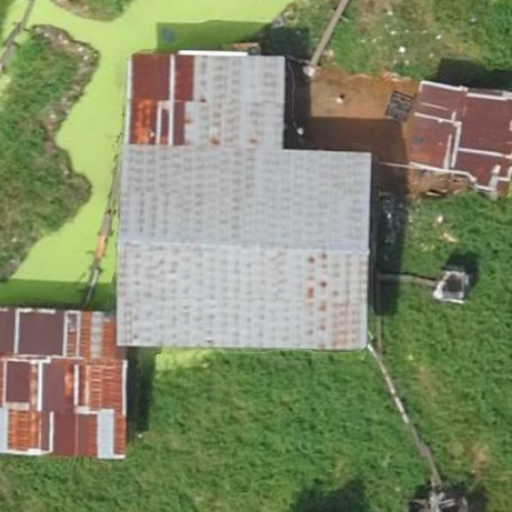
\includegraphics[width=\linewidth]{img/bld_1157971_raw.png}
    \caption{Segmentation patch}
\end{subfigure}
\hfill
\begin{subfigure}{0.32\textwidth}
    \centering
    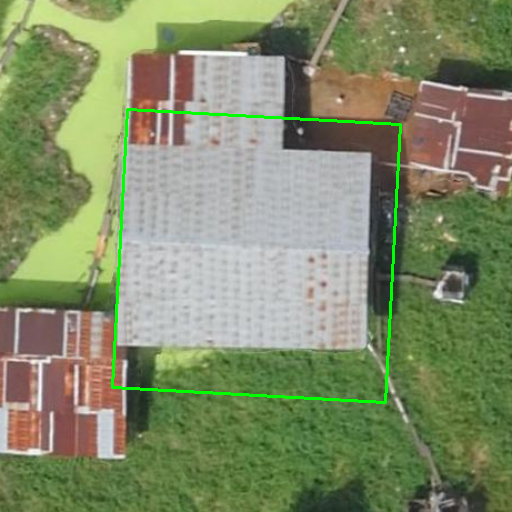
\includegraphics[width=\linewidth]{img/bld_1157971_clean.png}
    \caption{Assessment patch}
\end{subfigure}
\hfill
\begin{subfigure}{0.32\textwidth}
    \centering
    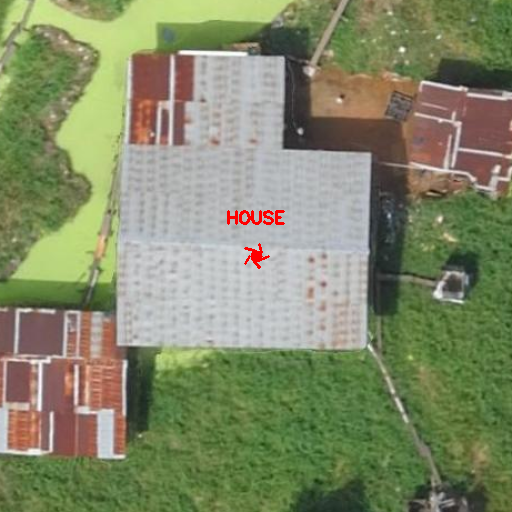
\includegraphics[width=\linewidth]{img/bld_1157971_debug.png}
    \caption{Prompt-reference patch}
\end{subfigure}

\caption{Example patch representations generated during preprocessing. The segmentation patch contains the original RGB imagery used for segmentation, the assessment patch overlays the original building footprint used for MLLM reasoning, and the prompt-reference patch includes a centroid reference marker used during prompt generation. All patches are normalized to a resolution of $512 \times 512$ pixels. Own illustration.}\label{fig:patch_types}

\end{figure}


During the refinement stage, patches may be re-extracted with an increased context factor to prevent boundary truncation effects. In the partial-house pipeline, additional localized sub-cropping is performed to isolate candidate building structures.


\section{MLLM-Based Quality Assessment}

\subsection{Model Configuration}

The MLLM-based quality assessment was performed using Qwen3-VL-8B-Instruct served through a vLLM backend on a remote GPU instance. Each request consisted of one image patch and a task-specific text prompt. Image inputs were provided at a standardized resolution of \(512 \times 512\) pixels. The model outputs were requested in a structured format and parsed into predefined fields used for routing, semantic error description, and prompt generation. Invalid or unparsable outputs were stored as failed outputs and excluded from downstream analyses where necessary.

\subsection{Structured QA Framework}

In the third stage of the workflow, a multimodal large language model (MLLM) is used to perform semantic quality assessment of the extracted building patch. The MLLM receives the assessment patch representation (image with polygon overlay) and produces a structured, machine-readable evaluation.

The assessment consists of three core reasoning tasks.

Because this stage determines the downstream routing and refinement strategy, the MLLM-based assessment was implemented as a sequence of task-specific prompts rather than as a single combined instruction. Each prompt addresses one clearly defined reasoning step and returns a structured JSON field that can be parsed automatically by the pipeline \citep{Zaid_prompt_decompisiton}. The full prompt content and JSON schema are documented in Appendix~\ref{app:mllm_prompts} and Appendix~\ref{app:mllm_json_schema}. Table~\ref{tab:mllm_reasoning_tasks} summarizes the main reasoning tasks used for semantic quality assessment.


\begin{table}[htb]
\centering
\small
\caption{MLLM reasoning tasks used for semantic quality assessment and routing. The prompt objectives are summarized from the operational prompts documented in Appendix~\ref{app:mllm_prompts}.}
\label{tab:mllm_reasoning_tasks}
\begin{tabular}{p{0.23\linewidth}p{0.46\linewidth}p{0.21\linewidth}}
\toprule
\textbf{Reasoning task} & \textbf{Prompt objective} & \textbf{Parsed output} \\
\midrule

Building presence &
Determine whether a visually identifiable roof or man-made building structure is present inside the overlaid polygon. &
\texttt{house\_present} \\

Footprint coverage &
Evaluate whether the polygon captures the majority of the visible roof or only a partial section of the building. &
\texttt{full\_house\_present} \\

Geometric error analysis &
Assess spatial misalignment and identify semantic geometry errors such as \texttt{SHAPE\_MISMATCH}, \texttt{MISSING\_PARTS}, and \texttt{EXTRA\_PARTS}. &
\texttt{error\_tags}, \texttt{error\_description} \\

\bottomrule
\end{tabular}
\end{table}

First, the model determines whether a visually identifiable roof structure is present within the polygon boundary. If no building structure is detected, the footprint is excluded from further processing and only the quality assessment result is stored. This prevents unnecessary refinement of non-building objects or false positives.

Second, the MLLM evaluates whether the polygon captures the majority of the visible building structure. This distinction is critical for downstream processing. If the polygon contains most of the building extent, refinement can be performed relative to the existing footprint. However, if the polygon captures only a small portion of the building, the initial bounding box derived from the footprint may be too restrictive. In such cases, a discovery-oriented refinement strategy must be applied to identify the full building extent prior to geometric correction.

Third, the model generates a semantic error assessment using a separate error-analysis prompt chain. The first prompt evaluates whether the polygon is spatially misaligned, the second prompt assigns predefined geometric error tags such as \texttt{SHAPE\_MISMATCH}, \texttt{MISSING\_PARTS}, and \texttt{EXTRA\_PARTS}, and the final prompt returns a short JSON field containing a human-readable error description. The resulting tags and description are stored with the MLLM decision output.

The MLLM tasks were intentionally split into smaller prompt chains instead of being handled in one combined instruction. This design follows the idea of task decomposition, where complex reasoning tasks are broken down into simpler subproblems that can be answered sequentially \citep{zhou2022least}. A similar strategy has also been shown to improve reliability in zero-shot visual question-answering by separating a complex visual task into individual sub-prompts \citep{Zaid_prompt_decompisiton}.

The result of this stage is a decision object containing four key attributes:

\begin{itemize}
    \item \texttt{house\_present}: Boolean indicator of building presence.
    \item \texttt{full\_house\_present}: Boolean or null indicator distinguishing full versus partial building coverage.
    \item \texttt{error\_description}: Structured semantic explanation of detected inconsistencies.
    \item \texttt{error\_tags}: List of predefined semantic geometry error categories assigned by the MLLM, such as \texttt{SHIFTED}, \texttt{SHAPE\_MISMATCH}, \texttt{MISSING\_PARTS}, \texttt{EXTRA\_PARTS}, or \texttt{OVERSIMPLIFIED}.
\end{itemize}

\subsection{Decision Logic and Routing}
\label{sec:decision_logic_routing}

Based on the decision object generated by the MLLM, buildings are routed into different refinement pipelines.

\begin{table}[htb]
\centering
\caption{Deterministic routing rules derived from the structured MLLM decision object.}
\label{tab:routing_rules}
\begin{tabular}{ccc}
\toprule
\texttt{house\_present} & \texttt{full\_house\_present} & \textbf{Pipeline} \\
\midrule
False & -- & None \\
True & True & FullHousePipeline \\
True & False / Null & PartialHousePipeline \\
\bottomrule
\end{tabular}
\end{table}

If the building is classified as partial or uncertain, a discovery-oriented refinement strategy is applied before geometric correction.

Figure~\ref{fig:partial_pipeline} illustrates this situation. In some cases the original footprint only covers a subset of the visible building structure. If the building were directly processed by the standard refinement pipeline, the prompts and bounding boxes provided to the segmentation model would restrict the segmentation to this limited region. As a result, the segmentation model would only refine the already detected subsection of the building instead of reconstructing the full structure.

To avoid this limitation, the system expands the spatial context around the building before applying the discovery-oriented refinement step. While the standard assessment and full-house refinement patches are generated with a context factor of 1.5, partial-house cases are re-extracted with a larger context factor of 4.0 (see Appendix \ref{app:core_parameters}). This enlarged window allows the discovery step to search beyond the limited original footprint extent and to identify additional visible building parts before the final SAM-based refinement is performed.

\begin{figure}[htbp]
\centering

\begin{subfigure}{0.45\textwidth}
    \centering
    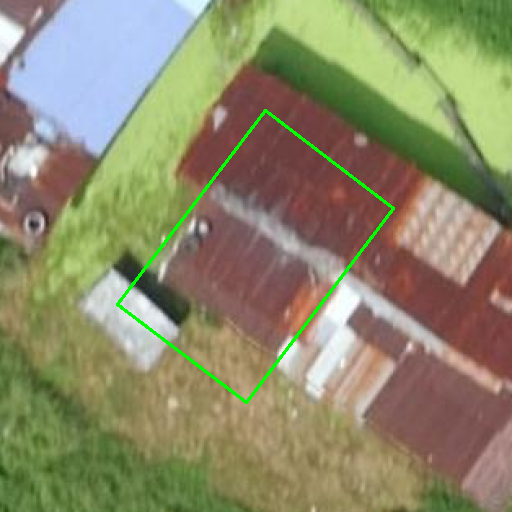
\includegraphics[width=\linewidth]{img/bld_1683655_clean.png}
    \caption{Initial footprint covering only part of the building}
\end{subfigure}
\hfill
\begin{subfigure}{0.45\textwidth}
    \centering
    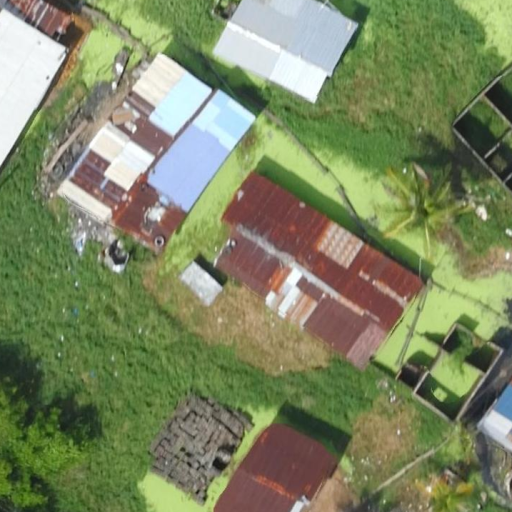
\includegraphics[width=\linewidth]{img/bld_1683655_partial_context.png}
    \caption{Expanded context used for structure discovery}
\end{subfigure}

\caption{Example of a partial building detection requiring context expansion. Own illustration.}
\label{fig:partial_pipeline}

\end{figure}

\section{Prompt Generation for the Visual Model}

Once a building has been routed into a refinement pipeline, spatial prompts must be generated to guide the segmentation model. Segment Anything (SAM) supports interactive prompting through a combination of positive points, negative points, and bounding boxes \citep{kirillov2023segment}.

In the proposed framework, prompt generation is performed automatically using the multimodal large language model (MLLM). The model receives the \emph{prompt-reference patch}, which contains the aerial image together with a visual reference marker indicating the centroid of the target building.

The prompt generation procedure produces two types of spatial constraints:

\begin{itemize}
\item \textbf{Positive points (inside points)} that lie on the roof surface of the target building.
\item \textbf{Negative points (outside points)} that lie outside the building.
\end{itemize}

The MLLM operates in a normalized coordinate system ranging from $(0,0)$ in the upper left corner to $(1000,1000)$ in the lower right corner of the image. The generated coordinates are then transformed into the pixel coordinate system of the patch.

Positive points are generated sequentially to ensure spatial coverage across the roof surface, while negative points help distinguish the building from surrounding structures.

In addition to point prompts, a bounding box derived from the original footprint geometry is used to constrain the search region of the segmentation model.

The resulting prompt configuration consists of:

\begin{itemize}
\item three positive roof points,
\item three negative background points,
\item one bounding box derived from the original footprint.
\end{itemize}

\section{Segmentation-Based Footprint Refinement}
\begin{wrapfigure}[40]{r}{0.45\textwidth}
\centering

\includegraphics[width=\linewidth]{Franzelin_Master/img/Flowchart_SAMStage.drawio.png}
\caption{Visual model refinement workflow. Own illustration.}
\label{fig:sam_stage}
\end{wrapfigure}
After the prompt generation stage, the building refinement process is performed using a visual segmentation foundation model. While the MLLM provides semantic interpretation and spatial guidance, the visual model is responsible for producing a geometrically precise building mask based on the underlying imagery.

The refinement stage consists of four main components:

\begin{itemize}
\item segmentation using text prompt,
\item segmentation using visual prompts,
\item iterative refinement and context expansion,
\item conversion of segmentation masks into geospatial vector geometries.
\end{itemize}

For the geometric refinement stage, the Segment Anything model family was used as the visual segmentation backbone \citep{kirillov2023segment, papersam3}. The final backend used in the implementation is specified below.

\subsection{Segmentation Model and Prompting Interfaces}

In this thesis, the term SAM-based refinement refers to the visual segmentation component used for prompt-based building-mask generation. The final implementation used a local SAM 3 checkpoint (\texttt{sam3.pt}) as the segmentation backend. Point- and box-guided refinement used the visual-prompt interface, while the text-prompted discovery step in the \textit{PartialHousePipeline} used the SAM 3 concept-prompted backend. 

In this work, the pretrained SAM-based backend was used without further architectural modifications. Preliminary experiments were conducted to fine-tune a previous model version (SAM 2) using building footprint data derived from two datasets: the Inria Aerial Image Labeling dataset and the SpaceNet 2 dataset for the Khartoum area. Approximately 1000 training patches were generated from these datasets. The two datasets represent different architectural contexts: the Inria dataset predominantly contains buildings from Western urban environments with pitched or heterogeneous roof structures, whereas the Khartoum dataset primarily consists of flat concrete roofs typical for dense settlements in Sudan.

Despite these experiments, the fine-tuned model did not improve segmentation performance. Instead, it showed clear signs of overfitting to specific roof textures and building patterns present in the training data. In particular, the model tended to over-segment roofs and to introduce artificial boundaries within single buildings, especially when roof materials varied within the same structure.

As a consequence, the model frequently produced overly detailed masks that fragmented individual buildings into multiple segments. This effect was particularly visible when applying the model to imagery outside the training regions, indicating poor generalization across different architectural styles and roof materials. Due to this degradation in generalization performance, the fine-tuning approach was abandoned and the pretrained SAM-based backend was used for the final workflow.

\subsection{Segmentation Model Usage in the Refinement Pipelines}
\label{sec:segmentation_model_usage}

The two refinement pipelines used in this work impose different requirements on the segmentation model. Consequently, the Segment Anything Model (SAM) is used in two distinct operational modes depending on the pipeline stage.

In the \textit{FullHousePipeline}, the model receives structured spatial prompts derived from the existing building footprint. These prompts consist of positive points placed on the roof surface, negative points placed outside the building, and a bounding box derived from the original polygon geometry. These prompts guide the segmentation model toward refining the existing footprint while preserving the approximate spatial extent of the building.

\begin{figure}[htb]
\centering

\begin{subfigure}{0.32\textwidth}
    \centering
    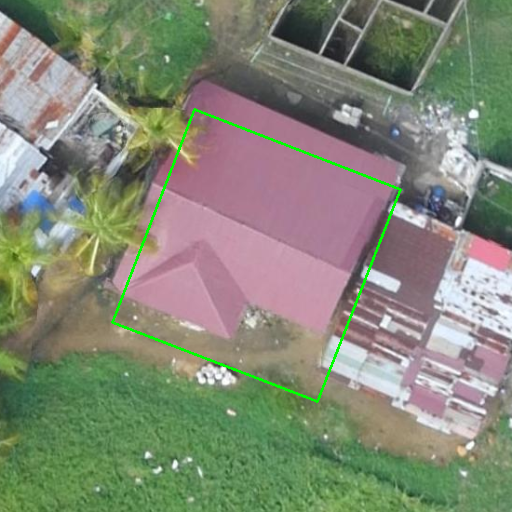
\includegraphics[width=\linewidth]{img/bld_0141916_clean.png}
    \caption{Original building footprint}
\end{subfigure}
\hfill
\begin{subfigure}{0.32\textwidth}
    \centering
    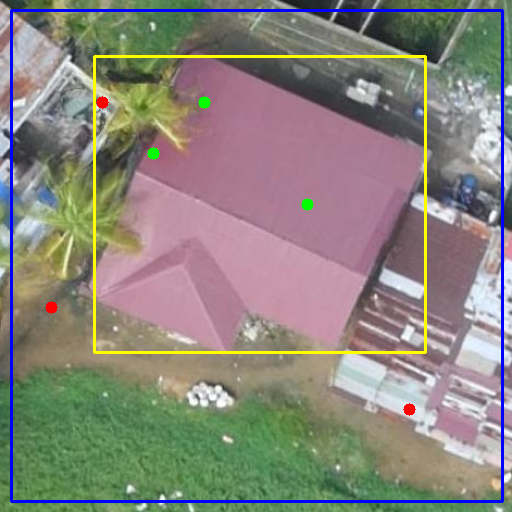
\includegraphics[width=\linewidth]{img/bld_0141916_sam_input.png}
    \caption{SAM prompt input}
\end{subfigure}
\hfill
\begin{subfigure}{0.32\textwidth}
    \centering
    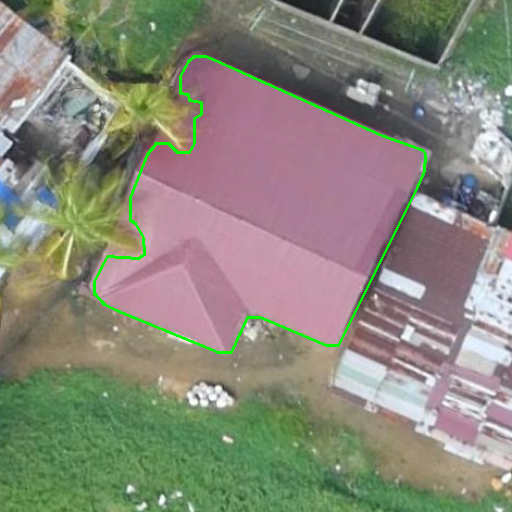
\includegraphics[width=\linewidth]{img/bld_0141916_sam.png}
    \caption{Refined segmentation result}
\end{subfigure}

\caption{FullHousePipeline refinement process. The existing building footprint provides spatial prompts that guide the segmentation model. Positive points, negative points, and a bounding box constrain the segmentation to refine the original footprint while preserving its approximate spatial extent. Own illustration.}
\label{fig:full_pipeline}

\end{figure}


In contrast, the \textit{PartialHousePipeline} addresses situations in which the original footprint captures only a subset of the visible building structure. In these cases, the polygon-derived bounding box may be too restrictive and would prevent the segmentation model from reconstructing the full building extent. Therefore, an additional detection step is introduced. Instead of restricting the model to the existing polygon, the text-prompted backend is used to identify all building structures within the image patch.

\begin{figure}[htb]
\centering

\begin{subfigure}[t]{0.24\textwidth}
    \vspace{0pt}
    \centering
    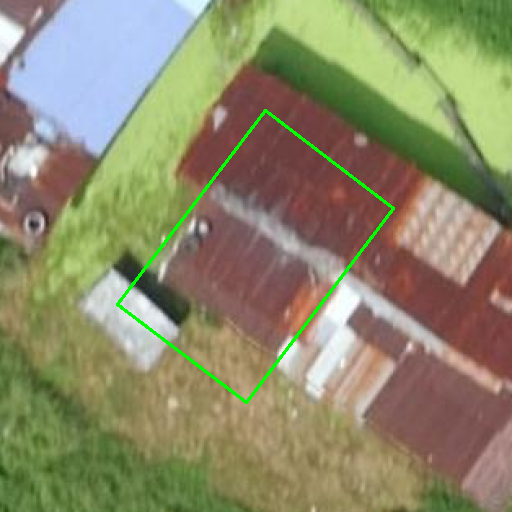
\includegraphics[width=\linewidth]{img/bld_1683655_clean.png}
    \caption{Incomplete footprint}
\end{subfigure}
\hfill
\begin{subfigure}[t]{0.24\textwidth}
    \vspace{0pt}
    \centering
    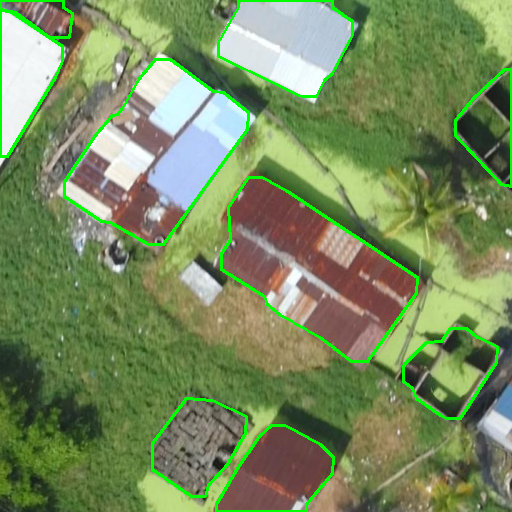
\includegraphics[width=\linewidth]{img/bld_1683655_detect_all_overlay.png}
    \caption{Text-prompted building discovery}
\end{subfigure}
\hfill
\begin{subfigure}[t]{0.24\textwidth}
    \vspace{0pt}
    \centering
    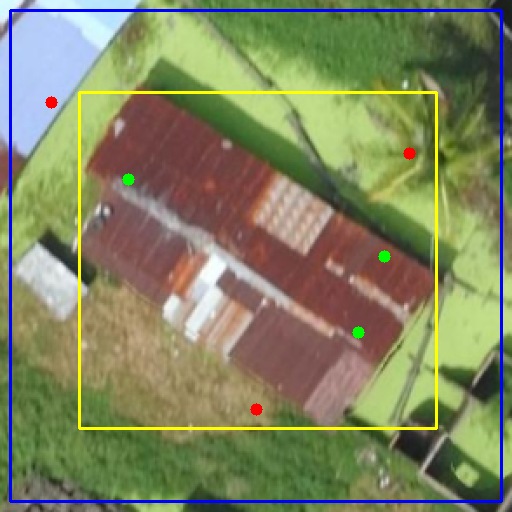
\includegraphics[width=\linewidth]{img/bld_1683655_sam_input.png}
    \caption{SAM prompt input}
\end{subfigure}
\hfill
\begin{subfigure}[t]{0.24\textwidth}
    \vspace{0pt}
    \centering
    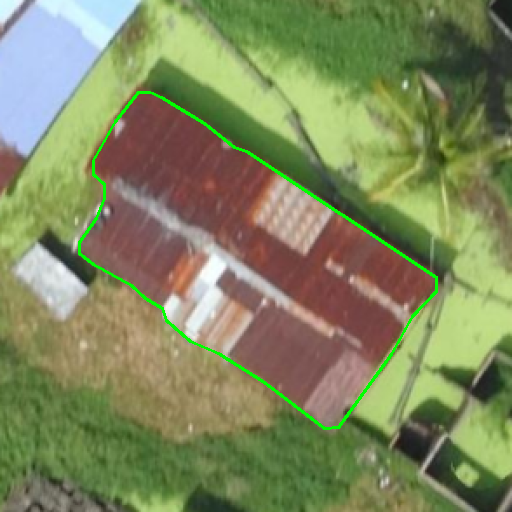
\includegraphics[width=\linewidth]{img/bld_1683655_sam.png}
    \caption{Refined building mask}
\end{subfigure}

\caption{PartialHousePipeline workflow. When the original footprint captures only part of the building, the spatial context is expanded and the segmentation model first performs a discovery step to identify the complete building structure before generating the final refined footprint. Own illustration.}

\label{fig:partial_pipeline_sam}

\end{figure}

For this discovery step, the implementation used the concept prompt ``roof''. The concept-prompted capability of SAM 3 allows the model to use semantic information in addition to spatial prompts.

This mechanism allows the model to detect complete building structures even when the initial footprint represents only a partial observation of the building. Once candidate roof regions have been identified, the candidate containing the original footprint centroid is selected; if no candidate contains the centroid, the nearest candidate centroid is used. The selected candidate is then passed to a local refinement crop where MLLM-generated positive and negative point prompts and the SAM-based visual-prompt backend produce the final refined building mask.
\subsection{Iterative Segmentation and Context Expansion}

Regardless of whether a building is routed through the \textit{FullHousePipeline} or the \textit{PartialHousePipeline}, the extracted patch ultimately passes through a common refinement stage in which the final building mask is generated using the SAM-based segmentation backend, as illustrated in Figure~\ref{fig:sam_stage}. In this stage, the multimodal large language model (MLLM) first generates spatial prompts in the form of positive and negative points. Together with an initial bounding box derived from the building footprint, these prompts serve as input for the visual segmentation backend. The segmentation process is performed iteratively. In the first iteration, a relatively large bounding box is used to ensure sufficient spatial context. After generating an initial mask, the bounding box is tightened to the extent of the predicted mask and the segmentation model is executed again to refine the segmentation. Where supported by the backend, segmentation logits from the previous iteration are passed to the next iteration. If the predicted polygon touches the boundary of the image patch, the system automatically extracts a larger patch to capture additional context. The refinement process was repeated for a maximum of three iterations or until no further context expansion was triggered.

\subsection{Polygon Extraction and Geometric Backprojection}

The segmentation model produces a binary mask in the \(512 \times 512\) patch coordinate system. This mask was converted into vector contours using OpenCV and subsequently into polygon geometries with Shapely. Small components and invalid geometries were removed or repaired before the polygon was transformed back into map coordinates. The inverse of the patch extraction transform was used to convert patch-pixel coordinates first to raster pixel coordinates and then to the raster CRS. The resulting polygon was stored in PostGIS together with the corresponding building identifier and run metadata.
\section{Post-processing}

The building polygons generated by the \textit{Segment Anything Model} (SAM) provide a strong initial representation of building footprints. However, due to the nature of image-based segmentation, the resulting geometries often contain inconsistencies that limit their direct usability for geospatial analysis. To address these issues, a structured post-processing pipeline is applied.

Three main types of geometric errors are observed:

\begin{itemize}
    \item \textbf{Fragmentation}: A single building may be represented by multiple adjacent or overlapping polygons. This is partly caused by inconsistencies in the source data and segmentation artifacts. These fragments are merged using geometric union operations combined with overlap-based grouping.
    \item \textbf{Irregular boundaries}: The segmentation process introduces small-scale noise along building edges, resulting in jagged or irregular raster-derived boundaries.
    \item \textbf{Tree occlusions}: Portions of building outlines are missing or distorted due to occlusion by vegetation. This leads to concave indentations or incomplete footprints and represents the most complex error type.
\end{itemize}

The post-processing pipeline addresses these issues step by step, combining geometric operations with simple assumptions about building shapes.

\subsection{Tree Occlusion}

Tree occlusions are handled by analyzing the spatial relationship between buildings and nearby trees. In the implementation, tree masks were generated with SAM 3 concept-prompted segmentation using the prompt ``tree'' and converted to polygon geometries before geometric repair. Let \(B\) be a building polygon and \(T\) the combined geometry of nearby trees.

First, a \textit{tree influence zone} is defined as a small area around the trees. This is done by slightly enlarging the tree geometry and subtracting a smaller inner buffer, where \(r_1\) and \(r_2\) denote the outer and inner tree-buffer radii, respectively:

\begin{equation}
Z_T = \operatorname{buffer}(T, r_1) \setminus \operatorname{buffer}(T, r_2).
\end{equation}

The tree influence zone \(Z_T\) represents the area where trees are likely to distort the building outline.

Next, possible occlusions are identified by intersecting this zone with the building boundary. The resulting candidate dent segments \(D_{\mathrm{cand}}\) are defined as:

\begin{equation}
D_{\mathrm{cand}} = \operatorname{boundary}(B) \cap Z_T.
\end{equation}

These candidate segments are split into smaller parts based on changes in direction. A segment is considered a candidate occlusion if it satisfies parameterized thresholds for distance to the tree boundary, minimum segment length, and deviation from a straight line.

Once such a dent is detected, the building shape is corrected. The idea is to reconstruct the missing part using the directions of the building edges before and after the dent.

Two simple cases are considered:

\begin{itemize}
    \item \textbf{Straight wall}: If both sides of the dent follow the same direction, the missing part is filled with a straight line.
    
    \item \textbf{Corner}: If the directions differ, the edges are extended until they meet, forming a new corner point.
\end{itemize}

To avoid unrealistic changes, the corrected polygon is only accepted if it remains similar to the original one. This is measured using the Intersection-over-Union (IoU), where \(B\) denotes the original polygon and \(B'\) the corrected polygon:

\begin{equation}
\operatorname{IoU}(B, B') =
\frac{\operatorname{area}(B \cap B')}{\operatorname{area}(B \cup B')}.
\end{equation}

The correction is applied only if this value is above a threshold.

This approach allows the reconstruction of building parts that were partially hidden by trees while preserving the overall shape of the building. The tree-occlusion component was custom-developed for this thesis. The main implementation parameters, including tree buffers, minimum overlap, and curvature thresholds, are listed in Appendix~\ref{app:core_parameters}.

\subsection{Polygon Regularization}
\label{sec:rectangularization}

After correcting tree occlusions, the building geometries are further refined to improve geometric regularity. The goal of this step is to reduce noise in the polygon boundaries while preserving the overall structure of the building.

Although this step is related to rectangularization, it does not enforce a single global orientation or force all buildings into idealized rectangular shapes.

As a baseline, the Python package \texttt{buildingregulariser} \citep{buildingregulariser} is used. However, this method was primarily developed for structured urban environments in highly planned regions, where buildings often follow consistent orientations and regular shapes. In such contexts, the algorithm applies strong assumptions, including a dominant global orientation and hard snapping of edges to predefined angles. These assumptions are less suitable for many regions in the Global South, where building layouts are often more irregular and do not follow a single dominant orientation. Applying a strict global alignment in such cases can lead to unrealistic distortions. To address this, a modified approach is used. Instead of deriving one global orientation for the full dataset, edge directions are analyzed separately for each polygon. The regularization first groups polygon edges into locally dominant direction clusters weighted by edge length and removes weak direction groups below a minimum weight ratio. The remaining dominant directions are ordered and constrained to orthogonal relationships. During angle enforcement, each sufficiently long edge is assigned to the nearest dominant direction group and then snapped fully to the nearest orthogonal target direction of that group if its deviation exceeds an adaptive tolerance. Very short edges are protected from this snapping step, and shorter retained edges use a larger tolerance. This makes the correction less intrusive for small boundary details while still reducing jagged mask-derived artifacts along the main building edges. After angle enforcement, the polygon is reconstructed and checked for geometric validity.

\section{Evaluation Strategy}
\label{sec:evaluation_strategy}

The evaluation approach is based on a manual assessment of building footprints across several regions in the Global South. The main objective is to determine whether the post-processed geometries produced by the pipeline improve upon the original input polygons. For each building, different aspects of geometric quality are examined, rather than relying on a single metric. The manual evaluation was based on visual agreement with the selected imagery rather than on independent cadastral ground truth.

To make the evaluation process efficient, a simple annotation tool was developed that allows quick navigation through the dataset and fast input of labels. The interface displayed the original polygon, the SAM-derived intermediate geometry, and the final post-processed geometry against the same imagery context (Figure~\ref{fig:evaluation_tool}). Ambiguous cases were rated conservatively according to the visible agreement between geometry and image evidence.

All manual ratings were assigned by the author using the same annotation interface and evaluation criteria. No independent second annotator was available; therefore, the labels should be interpreted as expert visual assessment rather than inter-annotator validated ground truth, and no inter-annotator agreement could be calculated.

In addition to the overall quality assessment, specific error types are recorded for both the original and the processed geometries. This enables an analysis of the dominant error sources before and after the pipeline. Furthermore, the manually assigned labels can be compared with the error descriptions generated by the multimodal model, allowing an assessment of how well the automated reasoning aligns with human evaluation.
\begin{figure}[htb]
	\centering  
	
\includegraphics[scale=0.5]{Franzelin_Master/img/evaluation_tool.png}
	\caption{Annotation interface used for manual evaluation of original, SAM-derived, and post-processed building geometries. Own illustration.}
	\label{fig:evaluation_tool}
\end{figure}
\subsection{Evaluation Criteria and Error Taxonomy}
\label{sec:evaluation_criteria_error_taxonomy}

The geometric quality of building footprints is assessed using an ordinal rating scheme with four categories:

\begin{itemize}
    \item \textbf{Perfect:} The geometry closely matches the visible building outline without relevant visible errors.
    \item \textbf{Good:} Minor deviations are present, but the overall structure is correct.
    \item \textbf{OK:} Noticeable errors exist, though the building remains recognizable.
    \item \textbf{Bad:} The geometry is severely inaccurate or does not represent the building.
\end{itemize}

For the improvement analysis, the ordinal classes were ordered as \textit{Bad} < \textit{OK} < \textit{Good} < \textit{Perfect}. A post-processed polygon was counted as improved if its final rating was higher than the original rating, unchanged if it remained in the same class, and degraded if it received a lower rating.

In addition to the overall rating, multiple error categories can be assigned to each building:

\begin{itemize}
    \item \texttt{SHIFTED}: Correct shape but incorrect spatial position.
    \item \texttt{SHAPE\_MISMATCH}: Geometry does not match the visible building form.
    \item \texttt{MISSING\_PARTS}: Parts of the building are not captured.
    \item \texttt{EXTRA\_PARTS}: Geometry includes non-building areas.
    \item \texttt{OVERSIMPLIFIED}: Shape lacks geometric detail.
\end{itemize}

Additionally, it is recorded whether post-processing introduces new errors:

\begin{itemize}
    \item \textbf{No:} No additional errors introduced.
    \item \textbf{Yes:} New geometric errors introduced during post-processing.
\end{itemize}

\subsection{Reference-based Switzerland Test}
\label{sec:switzerland_reference_test}

In addition to the main evaluation in the five Global South study areas, a small reference-based test was carried out in Switzerland. This test was not used as the primary evaluation of the proposed workflow, because the overall research focus of this thesis is on regions without reliable reference building datasets. Instead, it served as an additional plausibility check in an area where authoritative building geometries are available.

For this test, building polygons from the Microsoft Global ML Building Footprints dataset \citep{microsoft_globalmlbuildingfootprints} were selected in a SWISSIMAGE scene \citep{swisstopo_swissimage} and processed with the same building extraction and regularization workflow. The resulting regularized building polygons were then compared against Swiss TLM building geometries from the Swiss topographic landscape model swissTLM3D, which was used as the authoritative reference dataset \citep{swisstopo_swisstlm3d}. The evaluation was implemented in a separate ArcPy script and performed in the Swiss coordinate reference system CH1903+ / LV95 (EPSG:2056), so that all area and distance calculations were carried out in meters.

Because the regularization run for the Switzerland scene was interrupted, the evaluation was restricted to the subset of Microsoft buildings for which a corresponding regularized output was available. To reconstruct this processed subset, available regularized outputs were matched back to the Microsoft source polygons using a 1\,m spatial buffer. The corresponding TLM reference buildings were then selected around the processed Microsoft subset, also using a 1\,m buffer. This ensured that both the original Microsoft polygons and the regularized polygons were evaluated against the same reference subset.

Candidate-reference pairs were generated from polygon intersections and then matched greedily in descending IoU order, so that each candidate polygon and each TLM reference polygon could be used at most once. The evaluation was repeated for IoU thresholds of 0.10, 0.25 and 0.50. For each threshold, true positives, false positives and false negatives were counted, and precision, recall and F1-score were calculated. The same procedure was applied once to the regularized output and once to the corresponding Microsoft source polygons, allowing a direct comparison between the input footprints and the newly generated regularized result.

\subsection{Evaluation of Semantic Error Descriptions}
\label{sec:evaluation_semantic_error_descriptions}

As part of the workflow, semantic error descriptions were generated for each extracted building patch. The generation process consisted of multiple stages. First, a dedicated prompt determined whether the polygon was shifted relative to the visible building footprint. Subsequently, a second prompt was instructed to ignore positional displacement and instead identify additional geometric error categories. The prompt explicitly specified the semantic categories and provided instructions explaining when each category should be assigned.

In addition to the structured category-based approach, an unrestricted free-text prompt was investigated. This prompt generated short human-readable explanations describing the mismatch between the original polygon and the visible building structure in the aerial image.

The free-text descriptions cannot be directly compared to manually assigned semantic labels because they consist of unconstrained natural language. Therefore, a rule-based text analysis was implemented to map recurring words and short phrase patterns back to the semantic taxonomy used during manual evaluation.

The analysis was performed only for buildings for which both manual reference labels and Multi-modal LLM Quality Assessment (MLQA)-generated semantic descriptions were available. Placeholder outputs such as \textit{No building detected} and parsing-error messages were excluded from the analysis.

For each description, the generated sentence was converted to lower case and searched for predefined keywords and phrase patterns. If one or multiple patterns associated with a semantic category were identified, the corresponding category was assigned to the sentence. Multiple semantic categories could therefore be extracted from a single generated description.

\begin{table}[htb]
\centering
\caption{Keyword and phrase mapping used to extract semantic error categories from MLQA-generated free-text descriptions.}
\label{tab:semantic_sentence_keyword_mapping}
\begin{tabular}{p{0.28\linewidth}p{0.62\linewidth}}
\hline
\textbf{Extracted category} & \textbf{Indicative words and phrases} \\
\hline

\texttt{SHIFTED} &
shifted, shift, offset, misaligned, misalignment, displaced, not aligned, away from \\

\texttt{SHAPE\_MISMATCH} &
shape, form, wrong, incorrect, mismatch, does not match, not matching, not following, deviates, distorted, irregular \\

\texttt{OVERSIMPLIFIED} &
oversimplified, oversimplification, too simplified, over simplified, lacks detail, low detail, too simple, generalized \\

\texttt{MISSING\_PARTS} &
missing, omitted, incomplete, not fully cover, not fully enclose, not fully capture, does not fully cover, cut off, uncovered \\

\texttt{EXTRA\_PARTS} &
extra, includes, non-building, surrounding area, surrounding ground, vegetation, beyond, extending into, outside the building, too large, over-extends \\

\hline
\end{tabular}
\end{table}

In addition to the rule-based text analysis, a small manual qualitative evaluation of the generated sentences was carried out. A separate annotation interface was created for this purpose. The interface displayed the aerial image patch with the original polygon overlay and the corresponding MLQA-generated error description. The evaluator assigned one of four sentence-quality labels: \textit{Correct}, \textit{Partly correct}, \textit{Too vague}, or \textit{Wrong}. Initially, 50 examples per study area were exported for this evaluation. However, while reviewing the generated descriptions it became apparent that the model repeatedly produced very similar sentence structures and reused the same terms, especially references to missing and extra parts. Therefore, the qualitative evaluation was limited to approximately 100 sentences, as additional samples were unlikely to provide substantially new insight into the linguistic behavior of the model.

Moreover, to evaluate whether the MLLM-generated spatial prompts were consistent with successful building refinements, an additional point-in-polygon analysis was performed. The analysis was restricted to buildings that were manually rated as \textit{perfect} after processing, because these geometries represent the most reliable available approximation of the visible roof outline. Only full-house cases were included, since the secondary crop transformations required to reconstruct point coordinates for partial-house cases were not stored. The results should therefore not be generalized to the harder partial-house branch. For each analyzable building, the generated positive and negative prompt points were transformed back into map coordinates and tested against the corresponding final polygon.

\subsection{Building-to-Surrounding Contrast Analysis}
\label{sec:building_surrounding_contrast}

An additional image-based analysis was carried out to compare the visual contrast between buildings and their immediate surroundings in the five study areas. This analysis was included because low roof-ground contrast was expected to influence both the MLLM visibility decision and the SAM-based segmentation step.

For the automatic analysis, all post-processed buildings that received the manual quality label \textit{perfect} were selected. For each selected building, the final post-processed polygon was transformed into patch pixel coordinates and rasterized as the building mask. A local surrounding mask was then created by buffering the polygon outward by 48 pixels and subtracting an inner 4-pixel gap around the building boundary. The gap reduces direct edge effects caused by antialiasing, shadows, or small boundary misalignments. Pixels covered by neighboring building polygons were excluded from the surrounding mask so that the background measurement represented local ground context as far as possible. If the cleaned ring contained too few pixels, the remaining non-building pixels in the patch were used as a fallback background mask.

For each building, the mean brightness inside the building mask and inside the surrounding ring was calculated. The RGB values were first converted to linearized relative luminance so that the brightness comparison was not based directly on gamma-encoded image values. Denoting these luminance values by $Y_{\mathrm{building}}$ and $Y_{\mathrm{surrounding}}$, respectively, the final contrast value (C) used in the results is the absolute Weber contrast, a relative luminance-difference measure between a target and its background \citep{PelliBex2013}:


\begin{equation}
C = \left|
\frac{Y_{\mathrm{building}} - Y_{\mathrm{surrounding}}}
{Y_{\mathrm{surrounding}}}
\right|.
\end{equation}

This value describes how strongly the building differs in brightness from its local background, independent of whether the roof is brighter or darker than the surroundings. In addition, a simple texture-difference value was calculated using the same building and ring masks. The texture value combines three local image descriptors: Sobel gradient magnitude, absolute Laplacian response, and local standard deviation in a \(9 \times 9\) window. The Euclidean distance between the building texture descriptor and the surrounding texture descriptor was used as the final texture-difference value. It should be interpreted as a compact indicator of whether roof and background differ in edge density and local image variation.

The contrast and texture measures are used here as descriptive image statistics rather than as independent validation metrics.

\section{Implementation Details}

While the previous sections describe the methodological design of the workflow, this section summarizes the practical implementation choices required to execute the pipeline reproducibly. The implementation consists of a local Python-based geospatial processing environment, a PostgreSQL/PostGIS database for persistent spatial data management, and a remote GPU inference service for the multimodal model.

The processing code is organized as a modular Python project. The main entry point is \texttt{src/main.py}. Raster patch extraction is implemented in \texttt{patches/}, multimodal quality assessment in \texttt{mlqa/}, refinement logic in \texttt{pipelines/}, SAM-based segmentation in \texttt{sam/}, database operations in \texttt{db/}, and geometric post-processing in \texttt{postprocess/}. This structure separates processing responsibilities and allows individual components, such as the MLLM or segmentation backend, to be exchanged without modifying the complete workflow.

In addition to the evaluated per-building workflow, the code repository contains a tiled global-discovery extension that applies SAM 3 concept-prompted segmentation with the prompt ``roof'' to search for additional roof candidates. This component was treated as an exploratory extension and was not central to the reported quantitative evaluation.

Dependency management was handled using \texttt{uv}, a high-performance Python package and project manager \citep{uv_docs}. The main pipeline was executed in a project-specific Python 3.11 environment containing geospatial, computer vision, database, and model inference dependencies. Important libraries include \texttt{geopandas}, \texttt{rasterio}, \texttt{shapely}, \texttt{pyproj}, \texttt{opencv-python}, \texttt{torch}, \texttt{sqlalchemy}, \texttt{psycopg2}, and the OpenAI Python client. A separate virtual environment was used for the post-processing module, where the \texttt{buildingregulariser} package was linked as a locally editable dependency.

Persistent storage was implemented using PostgreSQL together with the PostGIS spatial extension, providing spatial indexing and geometry operations required for large-scale vector processing. Database access was configured through the environment variable \texttt{PG\_CONN}. The import scripts create the schema \texttt{src}, enable PostGIS, define required spatial tables, and generate spatial indexes.

The multimodal model was deployed separately from the local geospatial pipeline. Qwen3-VL-8B-Instruct was served on a RunPod GPU instance using \texttt{vLLM}, a high-throughput LLM serving framework designed for efficient inference and memory management through PagedAttention \citep{kwon2023pagedattention}. The model server exposes an OpenAI-compatible API, allowing the local Python code to communicate with the remote model through the standard OpenAI client interface. The RunPod instance is referenced through the environment variable \texttt{RUNPOD\_ID}, from which the endpoint URL is constructed. In this setup, the OpenAI client is used only as an API wrapper; the actual inference is performed by the self-hosted vLLM server.

Each pipeline run is assigned a unique \texttt{RUN\_ID}, which is written together with all detected geometries. This enables separation and comparison of different experimental runs within the database.


\Author{Jean Patrick Franzelin}
\chapter{Results}
\label{08_ergebnisse}

The workflow was applied to five study areas in the Global South introduced in Section~\ref{ch:study_area}. This chapter reports the pipeline coverage, changes in manually assessed polygon quality and error composition, geometric changes after refinement, the MLLM outputs, and the supplementary reference-based test in Switzerland. Unless stated otherwise, percentages refer to the latest manual evaluation for each of the 1,256 evaluated buildings. Percentages are rounded to one decimal place.

\section{Processed Dataset and Pipeline Coverage}

\subsection{MLQA Classification and Manual Evaluation Sample}

In total, 2,842 building polygons from the Google Open Buildings dataset were analyzed by the MLQA stage. The mutually exclusive routing classes comprised 1,283 cases classified as \textit{No visible}, 971 as \textit{Partial house}, and 588 as \textit{Full house}. Thus, 1,559 buildings were routed as visible partial- or full-house cases. A SAM-derived polygon was available for 1,518 buildings, a post-processed polygon for 1,352 buildings, and 1,256 buildings were included in the manual evaluation. The evaluated subset contains buildings for which the original and final geometries could be assigned and assessed consistently.

\begin{table}[htbp]
\centering
\caption{MLQA routing classes and manually evaluated subset by study area. The categories \textit{No visible}, \textit{Partial house}, and \textit{Full house} are mutually exclusive and sum to the MLQA input count.}
\label{tab:mlqa_overview}
\begin{tabular}{lrrrrr}
\toprule
Country & MLQA input & No visible & Partial house & Full house & Evaluated \\
\midrule
Liberia    & 616 & 111 & 324 & 181 & 380 \\
Mexico     & 500 & 167 & 224 & 109 & 261 \\
Mozambique & 600 & 424 & 122 & 54  & 167 \\
Nepal      & 626 & 359 & 198 & 69  & 192 \\
Niger      & 500 & 222 & 103 & 175 & 256 \\
\midrule
\textbf{Total} & \textbf{2,842} & \textbf{1,283} & \textbf{971} & \textbf{588} & \textbf{1,256} \\
\bottomrule
\end{tabular}
\end{table}

Cases classified as \textit{No visible} indicate that no corresponding visible building could be identified in the selected aerial or satellite imagery. The distinction between \textit{Partial house} and \textit{Full house}, and the resulting routing decision, are described in Section~\ref{sec:decision_logic_routing}.

\subsection{Pipeline Output Availability}

Table~\ref{tab:pipeline_dropoff} reports the number of unique buildings with outputs at each processing stage. The largest reduction occurred between MLQA input and available SAM output. Once a SAM-derived polygon was available, post-processed outputs were stored for 82.6--97.4\% of cases, depending on the study area. The manual evaluation was restricted to the comparable final subset.

\begin{table}[htbp]
\centering
\caption{Pipeline coverage by study area, showing unique buildings analyzed by MLQA, buildings with a SAM-derived output, buildings with a post-processed output, and manually evaluated buildings.}
\label{tab:pipeline_dropoff}
\begin{tabular}{lrrrrr}
\toprule
Country & MLQA input & SAM output & Post-processed & Evaluated & Post/SAM (\%) \\
\midrule
Liberia    & 616 & 483 & 399 & 380 & 82.6 \\
Mexico     & 500 & 331 & 291 & 261 & 87.9 \\
Mozambique & 600 & 176 & 169 & 167 & 96.0 \\
Nepal      & 626 & 263 & 235 & 192 & 89.4 \\
Niger      & 500 & 265 & 258 & 256 & 97.4 \\
\midrule
\textbf{Total} & \textbf{2,842} & \textbf{1,518} & \textbf{1,352} & \textbf{1,256} & \textbf{89.1} \\
\bottomrule
\end{tabular}
\end{table}

\section{Overall Quality Improvement}

\subsection{Transition from Original to Post-processed Quality}

Figure~\ref{fig:transition_heatmap} shows the transition between the original and post-processed manual ratings. Among the 581 buildings originally rated \textit{bad}, 292 received a final rating of \textit{perfect} and 153 a final rating of \textit{good}; 67 remained \textit{bad}. Among the 656 buildings originally rated \textit{ok}, 382 received a final rating of \textit{perfect} and 134 a rating of \textit{good}. Of the 19 originally \textit{good} buildings, 10 received a final rating of \textit{perfect}. No original polygon was rated \textit{perfect} in this subset.

\begin{figure}[htbp]
\centering

\includegraphics[scale=0.65]{Franzelin_Master/img/02_original_to_post_transition_heatmap.png}
\caption{Transition from original to post-processed manual quality ratings for the evaluated subset (\(n=1,256\)).}
\label{fig:transition_heatmap}
\end{figure}

Overall, the post-processed distribution comprised 116 \textit{bad}, 163 \textit{ok}, 293 \textit{good}, and 684 \textit{perfect} ratings.

\subsection{Improvement Rates by Study Area}

An improvement denotes a higher ordinal manual rating after post-processing, an unchanged case the same rating, and a degradation a lower rating. Across all study areas, 1,040 buildings improved (82.8\%), 164 remained unchanged (13.1\%), and 52 received a lower rating (4.1\%).

Niger had the highest improvement rate at 86.7\% (222/256), followed by Mozambique at 86.2\% (144/167) and Liberia at 86.1\% (327/380). The corresponding unchanged and degraded shares were 9.0\% and 4.3\% in Niger, 10.8\% and 3.0\% in Mozambique, and 12.6\% and 1.3\% in Liberia. Mexico improved in 77.0\% of cases (201/261), with 17.2\% unchanged and 5.7\% degraded. Nepal had an improvement rate of 76.0\% (146/192), with 15.6\% unchanged and 8.3\% degraded.

\begin{figure}[htbp]
\centering

\includegraphics[scale=0.65]{Franzelin_Master/img/02_country_improvement_rates.png}
\caption{Post-processing effect by study area for the manually evaluated subset (\(n=1,256\)). Improved, unchanged, and degraded indicate a higher, equal, or lower ordinal quality rating, respectively.}
\label{fig:country_improvement_rates}
\end{figure}

\subsection{Influence of Google Open Buildings Confidence}

The Google Open Buildings confidence score was compared with the original manual quality rating for all 1,256 evaluated buildings. Pearson's correlation was \(r=0.32\), while Spearman's rank correlation was \(\rho=0.31\). Higher confidence values therefore tended to coincide with higher original quality ratings, although the association was moderate.

\section{Changes in Error Composition}

\subsection{Dominant Errors in Original and Post-processed Geometries}

The error taxonomy is defined in Section~\ref{sec:evaluation_criteria_error_taxonomy}. Because multiple error categories could be assigned to one building, the percentages in Figure~\ref{fig:error_profile_by_location} are not mutually exclusive and can sum to more than 100\%.

\begin{figure}[htbp]
\centering

\includegraphics[width=\textwidth]{Franzelin_Master/img/02_error_categories_by_location_total.png}
\caption{Geometry error categories before and after post-processing by study area and for the complete evaluated subset (\(n=1,256\)). Categories are multi-label; percentages are therefore not mutually exclusive.}
\label{fig:error_profile_by_location}
\end{figure}

The most frequent original error was \texttt{SHIFTED}, assigned to 971 buildings (77.3\%). After post-processing, 54 buildings (4.3\%) retained this label. The original shares were highest in Mozambique (93.4\%), Niger (81.6\%), and Liberia (77.6\%); their post-processed shares were 3.6\%, 5.1\%, and 5.8\%, respectively.

The \texttt{SHAPE\_MISMATCH} category decreased from 474 buildings (37.7\%) to 164 (13.1\%). Nepal had the highest original and post-processed shares, at 61.5\% and 25.0\%. \texttt{OVERSIMPLIFIED} decreased from 171 cases (13.6\%) to 27 (2.1\%). In contrast, \texttt{MISSING\_PARTS} increased from 95 cases (7.6\%) to 198 (15.8\%), and \texttt{EXTRA\_PARTS} increased from 31 (2.5\%) to 134 (10.7\%). These increases are examined further in the Discussion.

The manual evaluation recorded a newly introduced post-processing error in 207 of 1,256 buildings (16.5\%). Overall, the largest observed change was the reduction in shifted polygons, while missing and extra parts became more frequent after post-processing.

\subsection{Detected Tree Context and New Post-processing Errors}

Detected tree context was derived from the ratio between the summed detected tree-mask area and the original building area. Cases with no tree mask were classified as \textit{no detected tree}; ratios up to 0.25 as \textit{low}, ratios above 0.25 and up to 1.0 as \textit{medium}, and ratios above 1.0 as \textit{high tree context}. These four classes are mutually exclusive.

Among 530 buildings without a detected tree, 13.4\% received a newly introduced error. Among the 726 buildings with a detected tree, the aggregated rate was 18.7\%. Within the mutually exclusive context classes, the rate ranged from 15.9\% for medium context to 23.0\% for high context. The binary association between detected trees and newly introduced errors was weak (\(\phi=0.07\)).

\begin{table}[htbp]
\centering
\caption{Newly introduced post-processing errors by mutually exclusive detected tree-context class for the evaluated subset (\(n=1,256\)).}
\label{tab:new_errors_tree_context}
\begin{tabular}{lrrrr}
\toprule
Tree context & n & New errors (\%) & Good/perfect (\%) & Missing parts (\%) \\
\midrule
No detected tree & 530 & 13.4 & 83.8 & 8.7 \\
Low              & 189 & 18.0 & 82.5 & 16.9 \\
Medium           & 302 & 15.9 & 75.8 & 21.9 \\
High             & 235 & 23.0 & 63.0 & 23.0 \\
\bottomrule
\end{tabular}
\end{table}

\section{Spatial Shift Analysis}

\subsection{Magnitude and Direction of Positional Corrections}

The shift analysis included the 971 buildings manually labelled \texttt{SHIFTED} in their original state. Centroid displacement was measured from the original polygon to the post-processed polygon using PostGIS geography distances in metres. The vector convention is positive \(dx\) towards the east and positive \(dy\) towards the north. Valid multipart geometries were included through the same centroid calculation.

\begin{figure}[htbp]
\centering

\includegraphics[scale=0.65]{Franzelin_Master/img/04_post_shift_vector_scatter_by_country.png}
\caption{Centroid displacement from the original to the post-processed polygon for buildings originally labelled \texttt{SHIFTED} (\(n=971\)); positive \(dx\) is east and positive \(dy\) is north.}
\label{fig:shift_vectors}
\end{figure}

Nepal showed the largest spread (\(n=124\), \(sd_{dx}=2.61\,\mathrm{m}\), \(sd_{dy}=3.80\,\mathrm{m}\), \(p90=8.88\,\mathrm{m}\)), followed by Mexico (\(n=187\), \(sd_{dx}=1.95\,\mathrm{m}\), \(sd_{dy}=2.94\,\mathrm{m}\), \(p90=7.20\,\mathrm{m}\)). Liberia had \(n=295\), \(sd_{dx}=1.29\,\mathrm{m}\), \(sd_{dy}=1.61\,\mathrm{m}\), and \(p90=4.68\,\mathrm{m}\). Mozambique (\(n=156\)) and Niger (\(n=209\)) showed lower component spreads: \(sd_{dx}=0.79\,\mathrm{m}\) and \(sd_{dy}=0.86\,\mathrm{m}\) in Mozambique, and \(sd_{dx}=0.85\,\mathrm{m}\) and \(sd_{dy}=0.78\,\mathrm{m}\) in Niger.

\section{Geometric Changes After Refinement}

\subsection{Area Preservation}

The signed area change was calculated as \(100(A_{post}/A_{original}-1)\); absolute area change uses the absolute value of this percentage. The scatterplot in Figure~\ref{fig:area_comparison} shows the original and post-processed areas with a 1:1 reference line. For readability, values above the 98th percentile of either axis are omitted from the figure, while the reported percentages use all 1,253 buildings with an available post-processed geometry.

\begin{figure}[htbp]
\centering

\includegraphics[scale=0.65]{Franzelin_Master/img/03_original_vs_post_area_scatter.png}
\caption{Original and post-processed building areas by study area. The dashed line is the 1:1 reference; values above the 98th percentile of either axis are omitted from the visualization.}
\label{fig:area_comparison}
\end{figure}

In Mozambique, 52.7\% of buildings remained within \(\pm10\%\) of their original area and 2.4\% became more than 50\% larger. The corresponding within-\(\pm10\%\) share was 39.1\% in Niger, 32.1\% in Liberia, 18.8\% in Mexico, and 13.0\% in Nepal. Buildings more than 50\% larger accounted for 20.2\% in Liberia, 31.8\% in Mexico, and 27.1\% in Nepal.

\subsection{Original, SAM-derived, and Post-processed Geometry Complexity}

Table~\ref{tab:stage_geometry_comparison} compares geometry size and vertex counts across stages. Vertex counts were calculated with \texttt{ST\_NPoints} on valid geometries and therefore include all rings, multipart components, and ring-closing coordinates. The three post-processed geometries unavailable for this calculation were all Liberia cases without a stored regularized geometry, resulting in \(n=1,253\) for the final stage.

\begin{table}[htbp]
\centering
\caption{Geometry characteristics of the original, SAM-derived, and post-processed polygons. Vertex counts include all coordinate points returned by \texttt{ST\_NPoints}.}
\label{tab:stage_geometry_comparison}
\begin{tabular}{lrrrr}
\toprule
Stage & n & Mean area (m$^2$) & Mean vertices & Median vertices \\
\midrule
Original Google & 1,256 & 73.02 & 5.27  & 5 \\
SAM-derived     & 1,256 & 77.65 & 40.81 & 39 \\
Post-processed  & 1,253 & 84.64 & 13.45 & 7 \\
\bottomrule
\end{tabular}
\end{table}

The SAM-derived polygons had the highest vertex counts. Post-processing reduced the mean and median vertex counts relative to the SAM-derived geometries, while the final counts remained above those of the original polygons.

\subsection{Full-house and Partial-house Cases}

Within the evaluated subset, 530 \textit{Full house} cases reached a \textit{good} or \textit{perfect} final rating in 79.6\% of cases and had a median absolute area change of 13.5\%. The 723 evaluated \textit{Partial house} cases reached these ratings in 76.3\% of cases and had a median absolute area change of 24.8\%.

\section{Building-to-Surrounding Contrast}

The image-based analysis described in Section~\ref{sec:building_surrounding_contrast} included all 684 buildings with a final rating of \textit{perfect}. Table~\ref{tab:building_surrounding_contrast} reports the median absolute Weber contrast after sRGB linearization and the median Euclidean difference between the building and surrounding texture descriptors.

\begin{table}[htbp]
\centering
\caption{Median building-to-surrounding metrics for all post-processed polygons rated \textit{perfect} (\(n=684\)). Contrast is the absolute linear Weber contrast; texture difference is the Euclidean distance between the building and surrounding texture descriptors.}
\label{tab:building_surrounding_contrast}
\begin{tabular}{lrrr}
\toprule
Country & n & Median Weber contrast & Median texture difference \\
\midrule
Liberia    & 195 & 0.838 & 28.0 \\
Mexico     & 125 & 1.662 & 16.7 \\
Mozambique & 120 & 0.246 & 16.8 \\
Nepal      & 68  & 0.678 & 23.1 \\
Niger      & 176 & 2.053 & 18.9 \\
\bottomrule
\end{tabular}
\end{table}

Mozambique had the lowest median Weber contrast, while Niger had the highest. Liberia had the highest median texture difference, followed by Nepal.

\section{Study Area Comparison}

Table~\ref{tab:country_summary} combines the quality, area, displacement, tree-context, and vertex-complexity indicators reported in the preceding sections. Nepal had the lowest \textit{good}/\textit{perfect} share (65.6\%), the largest median absolute area change (33.4\%), and the largest median centroid displacement (5.1\,m). Niger had the highest \textit{good}/\textit{perfect} share (85.9\%) and the smallest median displacement (1.7\,m). Mozambique had the smallest median absolute area change (9.0\%), while its medium/high tree-context share was the largest (68.9\%).

\begin{table}[htbp]
\centering
\caption{Study-area indicators for the manually evaluated subset. Area is the median absolute percentage change from the original polygon; shift is the median original-to-post-processed centroid displacement; tree context is the share classified as medium or high; vertex change is the increase in mean vertex count from original to post-processed geometry.}
\label{tab:country_summary}
\footnotesize
\begin{tabular}{lrrrrr}
\toprule
Country & \shortstack{Good/perfect\\(\%)} & \shortstack{Median absolute\\area change (\%)} & \shortstack{Median centroid\\displacement (m)} & \shortstack{Medium/high tree\\context (\%)} & \shortstack{Mean vertex\\increase (\%)} \\
\midrule
Liberia     & 79.5 & 16.0 & 3.1 & 35.5 & 154.6 \\
Mexico      & 72.4 & 30.7 & 3.7 & 63.6 & 162.1 \\
Mozambique  & 83.8 & 9.0  & 3.7 & 68.9 & 43.1 \\
Nepal       & 65.6 & 33.4 & 5.1 & 47.4 & 382.5 \\
Niger       & 85.9 & 14.7 & 1.7 & 11.7 & 45.0 \\
\bottomrule
\end{tabular}
\end{table}

\section{MLLM Outputs: Semantic Descriptions and Spatial Prompts}
\label{sec:results_mllm_outputs}

The semantic category outputs, free-text descriptions, and spatial point prompts were evaluated separately. Details of the prompts and extraction procedure are given in Section~\ref{sec:evaluation_semantic_error_descriptions}.

\subsection{Predefined Error Categories}
\label{sec:results_predefined_error_categories}

For 1,256 polygon pairs, the structured MLLM categories were compared with the manual labels for the original polygons. Exact category-set agreement occurred in 53 cases (4.2\%), with a mean Jaccard similarity of 0.408 and a median of 0.333. The manual evaluation assigned a mean of 1.39 labels per building, compared with 2.64 normalized MLQA labels.

The model output \texttt{MISALIGNED} was normalized to the manual category \texttt{SHIFTED}. The structured prompt requested \texttt{SHIFTED}, \texttt{SHAPE\_MISMATCH}, \texttt{MISSING\_PARTS}, and \texttt{EXTRA\_PARTS}; it did not request \texttt{OVERSIMPLIFIED}, which consequently had no structured MLQA predictions in this comparison.

\begin{table}[htbp]
\centering
\caption{Frequency of normalized structured MLQA categories and manual original-error labels for 1,256 polygon pairs. Categories are multi-label and percentages are shares of cases.}
\label{tab:semantic_category_comparison}
\begin{tabular}{lrr}
\toprule
Category & MLQA (\%) & Manual (\%) \\
\midrule
\texttt{SHIFTED}          & 97.6 & 77.3 \\
\texttt{SHAPE\_MISMATCH} & 90.8 & 37.7 \\
\texttt{OVERSIMPLIFIED}   & 0.0  & 13.6 \\
\texttt{MISSING\_PARTS}  & 2.5  & 7.6 \\
\texttt{EXTRA\_PARTS}    & 72.6 & 2.5 \\
\bottomrule
\end{tabular}
\end{table}

The largest frequency difference occurred for \texttt{EXTRA\_PARTS}, which was assigned in 72.6\% of MLQA outputs and 2.5\% of manual evaluations. \texttt{SHAPE\_MISMATCH} was also assigned more frequently by MLQA (90.8\%) than manually (37.7\%).

\subsection{Free-text Error Descriptions}
\label{sec:results_free_text_descriptions}

After excluding placeholder outputs and parsing failures, 1,250 cases remained for the rule-based extraction analysis. Exact agreement between the extracted and manual category sets occurred in 16 cases (1.3\%). The mean Jaccard similarity was 0.22 and the median was 0.25. The extracted descriptions contained a mean of 2.38 categories per case, compared with 1.39 manual categories.

Among the extracted categories, \texttt{SHIFTED} had the highest F1-score at 0.623 (precision 0.801, recall 0.509). \texttt{SHAPE\_MISMATCH} had an F1-score of 0.426. \texttt{MISSING\_PARTS} was extracted 898 times compared with 95 manual occurrences, and \texttt{EXTRA\_PARTS} was extracted 956 times compared with 31 manual occurrences. \texttt{OVERSIMPLIFIED} had one true-positive occurrence and an F1-score of 0.010.

The separate qualitative review retained the latest evaluation for 99 unique sentences. Eleven were rated \textit{correct}, 25 \textit{partly correct}, 37 \textit{too vague}, and 26 \textit{wrong}. Thus, 36 of 99 descriptions were at least partly correct.

\subsection{Spatial Accuracy of MLLM Point Prompts}
\label{sec:results_mllm_point_prompts}

The positive-point analysis included 320 full-house buildings with a final rating of \textit{perfect}. Of 960 positive points, 885 were inside or on the boundary of the corresponding polygon (92.19\%). All three positive points were correctly placed for 256 buildings (80.00\%). Agreement was 91.56\% for the first point, 96.56\% for the second, and 88.44\% for the third. Of the 75 positive points outside the polygon, 51 were within 0.5\,m of its boundary.

The negative-point analysis contained 963 points because one additional Mexico case retained a three-point negative prompt set but no corresponding positive prompt set. Of these negative points, 881 were outside the building polygon (91.48\%).

\section{Reference-based Switzerland Test}

The supplementary Switzerland test compared 425 workflow outputs and the corresponding 436 Microsoft source polygons against 488 TLM reference buildings. As described in Section~\ref{sec:switzerland_reference_test}, both candidate sets were evaluated against the same processed reference subset.

\begin{table}[htbp]
\centering
\caption{Reference-based evaluation of the processed Swiss subset against TLM geometries at three IoU thresholds.}
\label{tab:switzerland_reference_evaluation}
\begin{tabular}{llrrrrrr}
\toprule
Candidate & IoU & TP & FP & FN & Precision & Recall & F1 \\
\midrule
Workflow output & 0.10 & 387 & 38 & 101 & 0.911 & 0.793 & 0.848 \\
Workflow output & 0.25 & 377 & 48 & 111 & 0.887 & 0.773 & 0.826 \\
Workflow output & 0.50 & 340 & 85 & 148 & 0.800 & 0.697 & 0.745 \\
Microsoft       & 0.10 & 393 & 43 & 95  & 0.901 & 0.805 & 0.851 \\
Microsoft       & 0.25 & 383 & 53 & 105 & 0.878 & 0.785 & 0.829 \\
Microsoft       & 0.50 & 354 & 82 & 134 & 0.812 & 0.725 & 0.766 \\
\bottomrule
\end{tabular}
\end{table}

At IoU 0.50, the workflow output reached a precision of 0.800, recall of 0.697, and F1-score of 0.745. The Microsoft source polygons reached 0.812, 0.725, and 0.766, respectively. The Microsoft source polygons also had a slightly higher F1-score at IoU 0.10 and 0.25. According to this IoU-based comparison with the TLM reference geometries, the regularized workflow output did not improve over the Microsoft source polygons in this subset.


\Author{Jean Patrick Franzelin}
\chapter{Discussion}
\label{09_diskussion}

This thesis developed and evaluated a proof-of-concept workflow for improving existing building footprint polygons in selected study areas rather than generating a completely new building dataset from scratch. This distinction is important for geospatial data maintenance. In many practical settings, especially where automatically generated building datasets already exist, the central challenge is not only to detect buildings again, but to assess whether available polygons are fit for use and to selectively correct them where the imagery indicates geometric errors. This follows the broader idea of geodatabase updating, where modifying and improving existing spatial data can be more efficient than repeatedly creating new datasets \cite{Qin_changedetection}.

The work therefore connects two research directions that are often treated separately. On the one hand, building footprint extraction from high-resolution imagery has been studied extensively using classical deep learning architectures such as patch-based CNNs, fully convolutional networks, SegNet, and U-Net variants \cite{Luo_overviewbuioldingfootprint, rastogi2022automatic}. On the other hand, recent research on foundation models and multimodal large language models suggests that general-purpose models can support visual reasoning, spatial interpretation, and task-specific prompting without being trained from scratch for every individual application \cite{bommasani2022opportunitiesrisksfoundationmodels, wu2023multimodallargelanguagemodels, Yin_2024MLLM}. In this thesis, these ideas are combined in a two-stage workflow: a multimodal model first evaluates the plausibility of an existing footprint in relation to the image context, and a segmentation foundation model then refines the geometry where correction appears meaningful.

The specific contribution of this approach lies in the separation between semantic quality assessment and geometric correction. The MLLM is used for tasks that require contextual interpretation, such as deciding whether a visible roof is present, whether the original polygon covers the complete structure, and which type of error is likely present. SAM is then used for the image-driven segmentation task, where its prompt-based design allows the model to transform the MLLM output into a refined mask \cite{kirillov2023segment}. The final polygon is not simply the raw segmentation result, but the outcome of a controlled post-processing workflow that regularises and simplifies the segmentation into a usable vector geometry.

This setup is particularly relevant for data-scarce regions in the Global South. Global building footprint products such as Google Open Buildings provide important spatial information where authoritative datasets are often incomplete or unavailable \cite{sirko2021continentalscalebuildingdetectionhigh, CHAMBERLAIN2024102104}. At the same time, such automatically derived products contain characteristic errors related to shifts, incomplete footprints, merged structures, vegetation occlusion, and settlement-specific roof patterns. The discussion therefore focuses on whether the proposed combination of MLLM-based quality assessment, SAM-based refinement, and deterministic post-processing can meaningfully improve these existing polygons, where it fails, and what the results imply for the transferability of foundation-model-based geospatial quality assurance across different study areas.




\newpage




\Author{Jean Patrick Franzelin}
\chapter{Conclusion}
\label{ch:conclusion}

This thesis investigated whether recent vision and multimodal foundation models can support the quality assessment and selective refinement of existing building-footprint datasets in regions where authoritative reference data are often limited or unavailable. Instead of generating a new building dataset from scratch, the work focused on an update-oriented workflow: existing Google Open Buildings polygons were visually assessed against high-resolution OpenAerialMap imagery and, where necessary, refined using MLLM-guided prompting, SAM 3-based segmentation, and geometric post-processing.

The results show that this type of workflow can meaningfully improve the visual agreement between existing building polygons and the evaluated imagery. Across the five selected study areas, the workflow was applied to 2,842 Google Open Buildings polygons. Of these, 1,559 were routed as visible partial- or full-house cases, 1,518 produced a SAM-derived polygon, and 1,352 resulted in a post-processed output. The final manual evaluation included 1,256 buildings. Within this subset, 82.8\% of the evaluated polygons improved after post-processing, 13.1\% remained largely unchanged, and 4.1\% degraded. The share of polygons rated as \textit{good} or \textit{perfect} increased substantially after refinement, indicating that the proposed workflow was able to correct many visibly problematic building geometries.

With respect to the first research question, the results suggest that an MLLM can support visual quality assessment of existing vector-based building footprints, but mainly at a coarse decision-making level. The Qwen3 8B model was useful for identifying whether a building was visible, deciding whether a case should be processed as a full-house or partial-house example, and generating approximate positive and negative prompt points for SAM-based segmentation. The point-prompt evaluation showed that the spatial prompt generation worked reasonably well in successful full-house cases, with more than 90\% of positive and negative points being spatially consistent with the final building polygons. However, the MLLM was not reliable enough for fine-grained semantic error description. It struggled to consistently distinguish between shifted polygons, missing parts, extra parts, oversimplified outlines, and general shape mismatches. Therefore, the MLLM component should currently be understood as a useful routing and prompting aid, but not as a complete replacement for deterministic quality metrics or expert interpretation.

The second research question concerned the effectiveness of MLLM-generated prompts, SAM-based segmentation, and post-processing for improving selected building-footprint geometries. The strongest improvement was observed for positional displacement. The share of polygons classified as \texttt{SHIFTED} decreased from 77.3\% in the original Google Open Buildings polygons to 4.3\% after post-processing. \texttt{SHAPE\_MISMATCH} and \texttt{OVERSIMPLIFIED} errors were also reduced substantially. This demonstrates that the workflow was particularly effective for cases where an existing polygon already indicated the approximate presence of a building but did not align well with the visible roof structure. At the same time, the results also show that refinement introduced new challenges. The categories \texttt{MISSING\_PARTS} and \texttt{EXTRA\_PARTS} increased after processing, and new geometric errors were introduced in 16.5\% of the manually evaluated buildings. These errors were often related to ambiguous segmentation masks, vegetation, occlusion, complex roof structures, or the trade-off between preserving visual detail and producing clean GIS-ready vector geometries.

The third research question addressed transferability across different geographic regions, building morphologies, and imagery conditions. The workflow improved the majority of evaluated polygons in all five study areas, but the degree of improvement varied substantially. Niger and Mozambique achieved the strongest overall results, while Liberia produced strong but partly development-influenced results. Mexico and Nepal were more difficult cases, with lower final quality, larger area changes, and stronger increases in polygon complexity. These differences show that transferability is possible, but not uniform. The workflow performed best where buildings were visually separable and morphologically compact. It performed less reliably in areas with incremental housing, heterogeneous roof materials, dense structural complexity, vegetation, or ambiguous object boundaries. The supplementary Switzerland test further showed that the workflow is not automatically beneficial for already high-quality building datasets. In that case, the regularized outputs performed slightly worse than the existing Microsoft source polygons when compared against authoritative TLM geometries. This supports the interpretation that the method is most useful as a selective correction workflow for visibly problematic polygons, rather than as a universal improvement tool.

A central limitation of the thesis is that the evaluation was image-relative. The OpenAerialMap TIFF imagery used in this work was not necessarily identical to the imagery used to generate the original Google Open Buildings dataset. Therefore, the corrected polygons should be interpreted as geometrically improved with respect to the evaluated imagery, not necessarily as absolutely more accurate representations of the real-world building footprint at the time of analysis. This distinction is important because temporal differences, georeferencing uncertainty, image registration effects, and orthorectification differences may all contribute to apparent polygon-image mismatches.

Overall, the thesis demonstrates that multimodal and visual foundation models can contribute to local building-footprint quality assessment and refinement, but that they do not yet provide a fully automatic and reliable geospatial QA solution. The main contribution lies in showing how an existing global building dataset can be combined with MLLM-based visual reasoning, prompt generation, SAM-based segmentation, and vector post-processing in a modular workflow. The results indicate that such systems are especially promising when used in a human-in-the-loop setting: they can identify problematic polygons, generate candidate corrections, and support local mapping or database maintenance, while final decisions remain with human experts.

Future development should focus on more robust building regularization, better handling of occlusion and vegetation, systematic fine-tuning or evaluation of stronger spatial MLLMs, and closer integration into practical mapping workflows. If more capable geospatial foundation models become available, the MLLM component may improve substantially, especially for building detection, prompt placement, and semantic error interpretation. However, even with stronger models, reliable geospatial data maintenance will likely require a combination of visual AI, deterministic geometry checks, uncertainty communication, and human validation. In this sense, the workflow developed in this thesis should be understood not as a replacement for expert mapping, but as a step toward collaborative, AI-supported geospatial quality assessment for large-scale building-footprint datasets.




% ==========================================
% Literaturverzeichnis  einfügen
% ==========================================
%\bibliographystyle{unsrtdin}		%gibt den Zitierstyle an
\bibliographystyle{aiaa}
\bibliography{Literatur}\thispagestyle{rmplain}			%gibt alle Ihnhalte von JabRef aus
\label{bibpage}
\addcontentsline{toc}{chapter}{Literaturverzeichnis}
\cleardoublepage
%!Wichtig! JabRef fügt erst eine Litaratur aus dem Inhalt der Datenbank hinzu,
%wenn dieser im Text zitiert wird. Dazu muss man in JabRef einen Rechtsklick auf,
%das zu Zitierende Buch oder sonstiges machen. Anschließend die Maus auf Kopieren
%bewegen und im Drop-Down-Menu \cite{...}... auswählen. Als letztes noch "paste" an
%der gewünschent Stelle im Latex-Dokkument machen => fertig ist das Zitat.


% ============= Appendix einbinden ============= 
%\appendix		%Latex sagen, dass ab hier nur noch Anhänge kommen
\chapter*{Anhänge}\thispagestyle{rmplain}	%erstelltes Kapitel welches aber nicht im Inhaltsverzeichnis aufscheint 
\addcontentsline{toc}{chapter}{Anhänge}		%Inhaltsverzeichniseintrag ohne nummerierung für zuvor erstelles Kapitel erzeugen
\label{anhaenge}


\renewcommand{\thesection}{\Alph{section}}					%Sections mit Großbuchstaben durchnummerieren
\renewcommand{\thefigure}{\Alph{section}.\arabic{figure}}	%Art der Bildbeschriftung auf Buchstaben.Nummerierung.: ändern


\section{Name von Anhang A}\thispagestyle{rmplain}
\label{app_a}
\setcounter{figure}{0}		%Muss bei jeder neuen Section gesetzt werden, damit die Caption wieder bei eins zu nummerieren beginnt (z.B. A.1. A.2. ... B.1. B.2.)

%Der Anhang kommt hier rein
\begin{figure}[htb]
	\centering  
	\includegraphics[scale=0.5]{img/Lord_of_The_Rings_Logo.png}
	\caption{Lord of The Rings Logo}
	\label{fig:lotrl1}
\end{figure}

%\begin{figure}[htb]
%	\centering  
%	\includegraphics[scale=0.5]{img/Lord_of_The_Rings_Logo.png}
%	\caption{Lord of The Rings Logo}
%	\label{fig:lotrl2}
%\end{figure}
%\newpage

%%\section{Name von Anhang B}\thispagestyle{rmplain}
%\label{app_b}
%\setcounter{figure}{0}		%Muss bei jeder neuen Section gesetzt werden, damit die Caption wieder bei eins zu nummerieren beginnt (z.B. A.1. A.2. ... B.1. B.2.)

%Der Anhang kommt hier rein
%\begin{figure}[htb]
%%	\includegraphics[scale=0.5]{img/Lord_of_The_Rings_Logo.png}
	%\caption{Lord of The Rings Logo}
	%\label{fig:lotrl3}
%\end{figure}
\newpage
\end{document}